% ---------------------------------------------------------------------------
%  Venue switch.  iclr (default, official ICLR 2027 style included in this folder)
%                 neurips  -> needs the official neurips_2026.sty (or 2027) next to this file
%                 icml     -> needs the official icml2026.sty (or 2027); two-column, resize figures
% ---------------------------------------------------------------------------
\def\venue{iclr}

\documentclass{article}
\def\iclr{iclr}\def\neurips{neurips}\def\icml{icml}
\ifx\venue\iclr
  \usepackage{iclr2027_conference,times}
  %%%%% NEW MATH DEFINITIONS %%%%%

\usepackage{amsmath,amsfonts,bm}

% Mark sections of captions for referring to divisions of figures
\newcommand{\figleft}{{\em (Left)}}
\newcommand{\figcenter}{{\em (Center)}}
\newcommand{\figright}{{\em (Right)}}
\newcommand{\figtop}{{\em (Top)}}
\newcommand{\figbottom}{{\em (Bottom)}}
\newcommand{\captiona}{{\em (a)}}
\newcommand{\captionb}{{\em (b)}}
\newcommand{\captionc}{{\em (c)}}
\newcommand{\captiond}{{\em (d)}}

% Highlight a newly defined term
\newcommand{\newterm}[1]{{\bf #1}}


% Figure reference, lower-case.
\def\figref#1{figure~\ref{#1}}
% Figure reference, capital. For start of sentence
\def\Figref#1{Figure~\ref{#1}}
\def\twofigref#1#2{figures \ref{#1} and \ref{#2}}
\def\quadfigref#1#2#3#4{figures \ref{#1}, \ref{#2}, \ref{#3} and \ref{#4}}
% Section reference, lower-case.
\def\secref#1{section~\ref{#1}}
% Section reference, capital.
\def\Secref#1{Section~\ref{#1}}
% Reference to two sections.
\def\twosecrefs#1#2{sections \ref{#1} and \ref{#2}}
% Reference to three sections.
\def\secrefs#1#2#3{sections \ref{#1}, \ref{#2} and \ref{#3}}
% Reference to an equation, lower-case.
\def\eqref#1{equation~\ref{#1}}
% Reference to an equation, upper case
\def\Eqref#1{Equation~\ref{#1}}
% A raw reference to an equation---avoid using if possible
\def\plaineqref#1{\ref{#1}}
% Reference to a chapter, lower-case.
\def\chapref#1{chapter~\ref{#1}}
% Reference to an equation, upper case.
\def\Chapref#1{Chapter~\ref{#1}}
% Reference to a range of chapters
\def\rangechapref#1#2{chapters\ref{#1}--\ref{#2}}
% Reference to an algorithm, lower-case.
\def\algref#1{algorithm~\ref{#1}}
% Reference to an algorithm, upper case.
\def\Algref#1{Algorithm~\ref{#1}}
\def\twoalgref#1#2{algorithms \ref{#1} and \ref{#2}}
\def\Twoalgref#1#2{Algorithms \ref{#1} and \ref{#2}}
% Reference to a part, lower case
\def\partref#1{part~\ref{#1}}
% Reference to a part, upper case
\def\Partref#1{Part~\ref{#1}}
\def\twopartref#1#2{parts \ref{#1} and \ref{#2}}

\def\ceil#1{\lceil #1 \rceil}
\def\floor#1{\lfloor #1 \rfloor}
\def\1{\bm{1}}
\newcommand{\train}{\mathcal{D}}
\newcommand{\valid}{\mathcal{D_{\mathrm{valid}}}}
\newcommand{\test}{\mathcal{D_{\mathrm{test}}}}

\def\eps{{\epsilon}}


% Random variables
\def\reta{{\textnormal{$\eta$}}}
\def\ra{{\textnormal{a}}}
\def\rb{{\textnormal{b}}}
\def\rc{{\textnormal{c}}}
\def\rd{{\textnormal{d}}}
\def\re{{\textnormal{e}}}
\def\rf{{\textnormal{f}}}
\def\rg{{\textnormal{g}}}
\def\rh{{\textnormal{h}}}
\def\ri{{\textnormal{i}}}
\def\rj{{\textnormal{j}}}
\def\rk{{\textnormal{k}}}
\def\rl{{\textnormal{l}}}
% rm is already a command, just don't name any random variables m
\def\rn{{\textnormal{n}}}
\def\ro{{\textnormal{o}}}
\def\rp{{\textnormal{p}}}
\def\rq{{\textnormal{q}}}
\def\rr{{\textnormal{r}}}
\def\rs{{\textnormal{s}}}
\def\rt{{\textnormal{t}}}
\def\ru{{\textnormal{u}}}
\def\rv{{\textnormal{v}}}
\def\rw{{\textnormal{w}}}
\def\rx{{\textnormal{x}}}
\def\ry{{\textnormal{y}}}
\def\rz{{\textnormal{z}}}

% Random vectors
\def\rvepsilon{{\mathbf{\epsilon}}}
\def\rvtheta{{\mathbf{\theta}}}
\def\rva{{\mathbf{a}}}
\def\rvb{{\mathbf{b}}}
\def\rvc{{\mathbf{c}}}
\def\rvd{{\mathbf{d}}}
\def\rve{{\mathbf{e}}}
\def\rvf{{\mathbf{f}}}
\def\rvg{{\mathbf{g}}}
\def\rvh{{\mathbf{h}}}
\def\rvu{{\mathbf{i}}}
\def\rvj{{\mathbf{j}}}
\def\rvk{{\mathbf{k}}}
\def\rvl{{\mathbf{l}}}
\def\rvm{{\mathbf{m}}}
\def\rvn{{\mathbf{n}}}
\def\rvo{{\mathbf{o}}}
\def\rvp{{\mathbf{p}}}
\def\rvq{{\mathbf{q}}}
\def\rvr{{\mathbf{r}}}
\def\rvs{{\mathbf{s}}}
\def\rvt{{\mathbf{t}}}
\def\rvu{{\mathbf{u}}}
\def\rvv{{\mathbf{v}}}
\def\rvw{{\mathbf{w}}}
\def\rvx{{\mathbf{x}}}
\def\rvy{{\mathbf{y}}}
\def\rvz{{\mathbf{z}}}

% Elements of random vectors
\def\erva{{\textnormal{a}}}
\def\ervb{{\textnormal{b}}}
\def\ervc{{\textnormal{c}}}
\def\ervd{{\textnormal{d}}}
\def\erve{{\textnormal{e}}}
\def\ervf{{\textnormal{f}}}
\def\ervg{{\textnormal{g}}}
\def\ervh{{\textnormal{h}}}
\def\ervi{{\textnormal{i}}}
\def\ervj{{\textnormal{j}}}
\def\ervk{{\textnormal{k}}}
\def\ervl{{\textnormal{l}}}
\def\ervm{{\textnormal{m}}}
\def\ervn{{\textnormal{n}}}
\def\ervo{{\textnormal{o}}}
\def\ervp{{\textnormal{p}}}
\def\ervq{{\textnormal{q}}}
\def\ervr{{\textnormal{r}}}
\def\ervs{{\textnormal{s}}}
\def\ervt{{\textnormal{t}}}
\def\ervu{{\textnormal{u}}}
\def\ervv{{\textnormal{v}}}
\def\ervw{{\textnormal{w}}}
\def\ervx{{\textnormal{x}}}
\def\ervy{{\textnormal{y}}}
\def\ervz{{\textnormal{z}}}

% Random matrices
\def\rmA{{\mathbf{A}}}
\def\rmB{{\mathbf{B}}}
\def\rmC{{\mathbf{C}}}
\def\rmD{{\mathbf{D}}}
\def\rmE{{\mathbf{E}}}
\def\rmF{{\mathbf{F}}}
\def\rmG{{\mathbf{G}}}
\def\rmH{{\mathbf{H}}}
\def\rmI{{\mathbf{I}}}
\def\rmJ{{\mathbf{J}}}
\def\rmK{{\mathbf{K}}}
\def\rmL{{\mathbf{L}}}
\def\rmM{{\mathbf{M}}}
\def\rmN{{\mathbf{N}}}
\def\rmO{{\mathbf{O}}}
\def\rmP{{\mathbf{P}}}
\def\rmQ{{\mathbf{Q}}}
\def\rmR{{\mathbf{R}}}
\def\rmS{{\mathbf{S}}}
\def\rmT{{\mathbf{T}}}
\def\rmU{{\mathbf{U}}}
\def\rmV{{\mathbf{V}}}
\def\rmW{{\mathbf{W}}}
\def\rmX{{\mathbf{X}}}
\def\rmY{{\mathbf{Y}}}
\def\rmZ{{\mathbf{Z}}}

% Elements of random matrices
\def\ermA{{\textnormal{A}}}
\def\ermB{{\textnormal{B}}}
\def\ermC{{\textnormal{C}}}
\def\ermD{{\textnormal{D}}}
\def\ermE{{\textnormal{E}}}
\def\ermF{{\textnormal{F}}}
\def\ermG{{\textnormal{G}}}
\def\ermH{{\textnormal{H}}}
\def\ermI{{\textnormal{I}}}
\def\ermJ{{\textnormal{J}}}
\def\ermK{{\textnormal{K}}}
\def\ermL{{\textnormal{L}}}
\def\ermM{{\textnormal{M}}}
\def\ermN{{\textnormal{N}}}
\def\ermO{{\textnormal{O}}}
\def\ermP{{\textnormal{P}}}
\def\ermQ{{\textnormal{Q}}}
\def\ermR{{\textnormal{R}}}
\def\ermS{{\textnormal{S}}}
\def\ermT{{\textnormal{T}}}
\def\ermU{{\textnormal{U}}}
\def\ermV{{\textnormal{V}}}
\def\ermW{{\textnormal{W}}}
\def\ermX{{\textnormal{X}}}
\def\ermY{{\textnormal{Y}}}
\def\ermZ{{\textnormal{Z}}}

% Vectors
\def\vzero{{\bm{0}}}
\def\vone{{\bm{1}}}
\def\vmu{{\bm{\mu}}}
\def\vtheta{{\bm{\theta}}}
\def\va{{\bm{a}}}
\def\vb{{\bm{b}}}
\def\vc{{\bm{c}}}
\def\vd{{\bm{d}}}
\def\ve{{\bm{e}}}
\def\vf{{\bm{f}}}
\def\vg{{\bm{g}}}
\def\vh{{\bm{h}}}
\def\vi{{\bm{i}}}
\def\vj{{\bm{j}}}
\def\vk{{\bm{k}}}
\def\vl{{\bm{l}}}
\def\vm{{\bm{m}}}
\def\vn{{\bm{n}}}
\def\vo{{\bm{o}}}
\def\vp{{\bm{p}}}
\def\vq{{\bm{q}}}
\def\vr{{\bm{r}}}
\def\vs{{\bm{s}}}
\def\vt{{\bm{t}}}
\def\vu{{\bm{u}}}
\def\vv{{\bm{v}}}
\def\vw{{\bm{w}}}
\def\vx{{\bm{x}}}
\def\vy{{\bm{y}}}
\def\vz{{\bm{z}}}

% Elements of vectors
\def\evalpha{{\alpha}}
\def\evbeta{{\beta}}
\def\evepsilon{{\epsilon}}
\def\evlambda{{\lambda}}
\def\evomega{{\omega}}
\def\evmu{{\mu}}
\def\evpsi{{\psi}}
\def\evsigma{{\sigma}}
\def\evtheta{{\theta}}
\def\eva{{a}}
\def\evb{{b}}
\def\evc{{c}}
\def\evd{{d}}
\def\eve{{e}}
\def\evf{{f}}
\def\evg{{g}}
\def\evh{{h}}
\def\evi{{i}}
\def\evj{{j}}
\def\evk{{k}}
\def\evl{{l}}
\def\evm{{m}}
\def\evn{{n}}
\def\evo{{o}}
\def\evp{{p}}
\def\evq{{q}}
\def\evr{{r}}
\def\evs{{s}}
\def\evt{{t}}
\def\evu{{u}}
\def\evv{{v}}
\def\evw{{w}}
\def\evx{{x}}
\def\evy{{y}}
\def\evz{{z}}

% Matrix
\def\mA{{\bm{A}}}
\def\mB{{\bm{B}}}
\def\mC{{\bm{C}}}
\def\mD{{\bm{D}}}
\def\mE{{\bm{E}}}
\def\mF{{\bm{F}}}
\def\mG{{\bm{G}}}
\def\mH{{\bm{H}}}
\def\mI{{\bm{I}}}
\def\mJ{{\bm{J}}}
\def\mK{{\bm{K}}}
\def\mL{{\bm{L}}}
\def\mM{{\bm{M}}}
\def\mN{{\bm{N}}}
\def\mO{{\bm{O}}}
\def\mP{{\bm{P}}}
\def\mQ{{\bm{Q}}}
\def\mR{{\bm{R}}}
\def\mS{{\bm{S}}}
\def\mT{{\bm{T}}}
\def\mU{{\bm{U}}}
\def\mV{{\bm{V}}}
\def\mW{{\bm{W}}}
\def\mX{{\bm{X}}}
\def\mY{{\bm{Y}}}
\def\mZ{{\bm{Z}}}
\def\mBeta{{\bm{\beta}}}
\def\mPhi{{\bm{\Phi}}}
\def\mLambda{{\bm{\Lambda}}}
\def\mSigma{{\bm{\Sigma}}}

% Tensor
\DeclareMathAlphabet{\mathsfit}{\encodingdefault}{\sfdefault}{m}{sl}
\SetMathAlphabet{\mathsfit}{bold}{\encodingdefault}{\sfdefault}{bx}{n}
\newcommand{\tens}[1]{\bm{\mathsfit{#1}}}
\def\tA{{\tens{A}}}
\def\tB{{\tens{B}}}
\def\tC{{\tens{C}}}
\def\tD{{\tens{D}}}
\def\tE{{\tens{E}}}
\def\tF{{\tens{F}}}
\def\tG{{\tens{G}}}
\def\tH{{\tens{H}}}
\def\tI{{\tens{I}}}
\def\tJ{{\tens{J}}}
\def\tK{{\tens{K}}}
\def\tL{{\tens{L}}}
\def\tM{{\tens{M}}}
\def\tN{{\tens{N}}}
\def\tO{{\tens{O}}}
\def\tP{{\tens{P}}}
\def\tQ{{\tens{Q}}}
\def\tR{{\tens{R}}}
\def\tS{{\tens{S}}}
\def\tT{{\tens{T}}}
\def\tU{{\tens{U}}}
\def\tV{{\tens{V}}}
\def\tW{{\tens{W}}}
\def\tX{{\tens{X}}}
\def\tY{{\tens{Y}}}
\def\tZ{{\tens{Z}}}


% Graph
\def\gA{{\mathcal{A}}}
\def\gB{{\mathcal{B}}}
\def\gC{{\mathcal{C}}}
\def\gD{{\mathcal{D}}}
\def\gE{{\mathcal{E}}}
\def\gF{{\mathcal{F}}}
\def\gG{{\mathcal{G}}}
\def\gH{{\mathcal{H}}}
\def\gI{{\mathcal{I}}}
\def\gJ{{\mathcal{J}}}
\def\gK{{\mathcal{K}}}
\def\gL{{\mathcal{L}}}
\def\gM{{\mathcal{M}}}
\def\gN{{\mathcal{N}}}
\def\gO{{\mathcal{O}}}
\def\gP{{\mathcal{P}}}
\def\gQ{{\mathcal{Q}}}
\def\gR{{\mathcal{R}}}
\def\gS{{\mathcal{S}}}
\def\gT{{\mathcal{T}}}
\def\gU{{\mathcal{U}}}
\def\gV{{\mathcal{V}}}
\def\gW{{\mathcal{W}}}
\def\gX{{\mathcal{X}}}
\def\gY{{\mathcal{Y}}}
\def\gZ{{\mathcal{Z}}}

% Sets
\def\sA{{\mathbb{A}}}
\def\sB{{\mathbb{B}}}
\def\sC{{\mathbb{C}}}
\def\sD{{\mathbb{D}}}
% Don't use a set called E, because this would be the same as our symbol
% for expectation.
\def\sF{{\mathbb{F}}}
\def\sG{{\mathbb{G}}}
\def\sH{{\mathbb{H}}}
\def\sI{{\mathbb{I}}}
\def\sJ{{\mathbb{J}}}
\def\sK{{\mathbb{K}}}
\def\sL{{\mathbb{L}}}
\def\sM{{\mathbb{M}}}
\def\sN{{\mathbb{N}}}
\def\sO{{\mathbb{O}}}
\def\sP{{\mathbb{P}}}
\def\sQ{{\mathbb{Q}}}
\def\sR{{\mathbb{R}}}
\def\sS{{\mathbb{S}}}
\def\sT{{\mathbb{T}}}
\def\sU{{\mathbb{U}}}
\def\sV{{\mathbb{V}}}
\def\sW{{\mathbb{W}}}
\def\sX{{\mathbb{X}}}
\def\sY{{\mathbb{Y}}}
\def\sZ{{\mathbb{Z}}}

% Entries of a matrix
\def\emLambda{{\Lambda}}
\def\emA{{A}}
\def\emB{{B}}
\def\emC{{C}}
\def\emD{{D}}
\def\emE{{E}}
\def\emF{{F}}
\def\emG{{G}}
\def\emH{{H}}
\def\emI{{I}}
\def\emJ{{J}}
\def\emK{{K}}
\def\emL{{L}}
\def\emM{{M}}
\def\emN{{N}}
\def\emO{{O}}
\def\emP{{P}}
\def\emQ{{Q}}
\def\emR{{R}}
\def\emS{{S}}
\def\emT{{T}}
\def\emU{{U}}
\def\emV{{V}}
\def\emW{{W}}
\def\emX{{X}}
\def\emY{{Y}}
\def\emZ{{Z}}
\def\emSigma{{\Sigma}}

% entries of a tensor
% Same font as tensor, without \bm wrapper
\newcommand{\etens}[1]{\mathsfit{#1}}
\def\etLambda{{\etens{\Lambda}}}
\def\etA{{\etens{A}}}
\def\etB{{\etens{B}}}
\def\etC{{\etens{C}}}
\def\etD{{\etens{D}}}
\def\etE{{\etens{E}}}
\def\etF{{\etens{F}}}
\def\etG{{\etens{G}}}
\def\etH{{\etens{H}}}
\def\etI{{\etens{I}}}
\def\etJ{{\etens{J}}}
\def\etK{{\etens{K}}}
\def\etL{{\etens{L}}}
\def\etM{{\etens{M}}}
\def\etN{{\etens{N}}}
\def\etO{{\etens{O}}}
\def\etP{{\etens{P}}}
\def\etQ{{\etens{Q}}}
\def\etR{{\etens{R}}}
\def\etS{{\etens{S}}}
\def\etT{{\etens{T}}}
\def\etU{{\etens{U}}}
\def\etV{{\etens{V}}}
\def\etW{{\etens{W}}}
\def\etX{{\etens{X}}}
\def\etY{{\etens{Y}}}
\def\etZ{{\etens{Z}}}

% The true underlying data generating distribution
\newcommand{\pdata}{p_{\rm{data}}}
% The empirical distribution defined by the training set
\newcommand{\ptrain}{\hat{p}_{\rm{data}}}
\newcommand{\Ptrain}{\hat{P}_{\rm{data}}}
% The model distribution
\newcommand{\pmodel}{p_{\rm{model}}}
\newcommand{\Pmodel}{P_{\rm{model}}}
\newcommand{\ptildemodel}{\tilde{p}_{\rm{model}}}
% Stochastic autoencoder distributions
\newcommand{\pencode}{p_{\rm{encoder}}}
\newcommand{\pdecode}{p_{\rm{decoder}}}
\newcommand{\precons}{p_{\rm{reconstruct}}}

\newcommand{\laplace}{\mathrm{Laplace}} % Laplace distribution

\newcommand{\E}{\mathbb{E}}
\newcommand{\Ls}{\mathcal{L}}
\newcommand{\R}{\mathbb{R}}
\newcommand{\emp}{\tilde{p}}
\newcommand{\lr}{\alpha}
\newcommand{\reg}{\lambda}
\newcommand{\rect}{\mathrm{rectifier}}
\newcommand{\softmax}{\mathrm{softmax}}
\newcommand{\sigmoid}{\sigma}
\newcommand{\softplus}{\zeta}
\newcommand{\KL}{D_{\mathrm{KL}}}
\newcommand{\Var}{\mathrm{Var}}
\newcommand{\standarderror}{\mathrm{SE}}
\newcommand{\Cov}{\mathrm{Cov}}
% Wolfram Mathworld says $L^2$ is for function spaces and $\ell^2$ is for vectors
% But then they seem to use $L^2$ for vectors throughout the site, and so does
% wikipedia.
\newcommand{\normlzero}{L^0}
\newcommand{\normlone}{L^1}
\newcommand{\normltwo}{L^2}
\newcommand{\normlp}{L^p}
\newcommand{\normmax}{L^\infty}

\newcommand{\parents}{Pa} % See usage in notation.tex. Chosen to match Daphne's book.

\DeclareMathOperator*{\argmax}{arg\,max}
\DeclareMathOperator*{\argmin}{arg\,min}

\DeclareMathOperator{\sign}{sign}
\DeclareMathOperator{\Tr}{Tr}
\let\ab\allowbreak

\else\ifx\venue\neurips
  \usepackage[eandd]{neurips_2026}
\else
  \usepackage{icml2026}
\fi\fi

\usepackage[utf8]{inputenc}
\usepackage[T1]{fontenc}
\usepackage{hyperref}
\usepackage{url}
\usepackage{amsmath,amssymb,amsthm}
\usepackage{graphicx}
\usepackage{booktabs}
\usepackage{multirow}
\usepackage{enumitem}
\usepackage{xcolor}
\usepackage{microtype}
\usepackage{placeins}
\usepackage[capitalise,nameinlink]{cleveref}
\hypersetup{colorlinks=true, linkcolor=black, citecolor=[HTML]{1c5cab}, urlcolor=[HTML]{1c5cab}}

\newtheorem{proposition}{Proposition}
\crefname{proposition}{Proposition}{Propositions}
\newcommand{\doi}[1]{\href{https://doi.org/#1}{doi:#1}}
\newcommand{\numBTaccAll}{80\%}
\newcommand{\numBTaccClean}{60\%}
\newcommand{\numBTaccFlag}{99\%}
\newcommand{\numBTcross}{2.0\%}
\newcommand{\numBTexact}{88}
\newcommand{\numBTexactPct}{22\%}
\newcommand{\numBTflag}{200}
\newcommand{\numBTflagHi}{152}
\newcommand{\numBTflagHiPct}{39\%}
\newcommand{\numBTflagPct}{51\%}
\newcommand{\numBTnnClean}{59\%}
\newcommand{\numBTnnFlag}{100\%}
\newcommand{\numBTntest}{394}
\newcommand{\numBTyes}{40/40}
\newcommand{\numCifarText}{AugLeak flags 274 CIFAR-10 test images (2.7\%) at $\alpha=10^{-2}$ and 118 (1.2\%) at $\alpha=10^{-3}$, against the $3.3\%$ that \citet{barz2020cifair} found with learned retrieval and manual inspection; 55 of the $60$ top-ranked pairs are near-duplicates, and 1-NN scores 94.9\% on images flagged at $\alpha=10^{-3}$ against 73.2\% on the rest.}
\newcommand{\numCovidKnnGap}{8.8}
\newcommand{\numCovidLpGap}{5.6}
\newcommand{\numCovidQ}{56.9\%}
\newcommand{\numDetCmediumallAP}{0.71}
\newcommand{\numDetCmediumallFL}{0.1\%}
\newcommand{\numDetCmediumallHit}{70\%}
\newcommand{\numDetCmediumallResid}{85\%}
\newcommand{\numDetCmediuminvAP}{0.66}
\newcommand{\numDetCmediuminvFL}{0.4\%}
\newcommand{\numDetCmediuminvHit}{74\%}
\newcommand{\numDetCmediuminvResid}{82\%}
\newcommand{\numDetCmediumphashdfourAP}{0.04}
\newcommand{\numDetCmediumphashdfourFL}{0.0\%}
\newcommand{\numDetCmediumphashdfourHit}{6\%}
\newcommand{\numDetCmediumphashdfourResid}{100\%}
\newcommand{\numDetCmediumpixAP}{0.42}
\newcommand{\numDetCmediumpixFL}{0.0\%}
\newcommand{\numDetCmediumpixHit}{26\%}
\newcommand{\numDetCmediumpixResid}{99\%}
\newcommand{\numDetCmediumsemAP}{0.62}
\newcommand{\numDetCmediumsemFL}{0.5\%}
\newcommand{\numDetCmediumsemHit}{43\%}
\newcommand{\numDetCmediumsemResid}{95\%}
\newcommand{\numDetCmediumstructAP}{0.48}
\newcommand{\numDetCmediumstructFL}{0.0\%}
\newcommand{\numDetCmediumstructHit}{23\%}
\newcommand{\numDetCmediumstructResid}{100\%}
\newcommand{\numDetCstrongallAP}{0.11}
\newcommand{\numDetCstrongallFL}{0.1\%}
\newcommand{\numDetCstrongallHit}{9\%}
\newcommand{\numDetCstrongallResid}{100\%}
\newcommand{\numDetCstronginvAP}{0.07}
\newcommand{\numDetCstronginvFL}{0.2\%}
\newcommand{\numDetCstronginvHit}{9\%}
\newcommand{\numDetCstronginvResid}{100\%}
\newcommand{\numDetCstrongphashdfourAP}{0.01}
\newcommand{\numDetCstrongphashdfourFL}{0.0\%}
\newcommand{\numDetCstrongphashdfourHit}{1\%}
\newcommand{\numDetCstrongphashdfourResid}{100\%}
\newcommand{\numDetCstrongpixAP}{0.09}
\newcommand{\numDetCstrongpixFL}{0.0\%}
\newcommand{\numDetCstrongpixHit}{4\%}
\newcommand{\numDetCstrongpixResid}{100\%}
\newcommand{\numDetCstrongsemAP}{0.07}
\newcommand{\numDetCstrongsemFL}{0.1\%}
\newcommand{\numDetCstrongsemHit}{5\%}
\newcommand{\numDetCstrongsemResid}{100\%}
\newcommand{\numDetCstrongstructAP}{0.12}
\newcommand{\numDetCstrongstructFL}{0.0\%}
\newcommand{\numDetCstrongstructHit}{3\%}
\newcommand{\numDetCstrongstructResid}{100\%}
\newcommand{\numDetCweakallAP}{1.00}
\newcommand{\numDetCweakallFL}{1.0\%}
\newcommand{\numDetCweakallHit}{100\%}
\newcommand{\numDetCweakallResid}{0\%}
\newcommand{\numDetCweakinvAP}{1.00}
\newcommand{\numDetCweakinvFL}{2.2\%}
\newcommand{\numDetCweakinvHit}{100\%}
\newcommand{\numDetCweakinvResid}{0\%}
\newcommand{\numDetCweakphashdfourAP}{1.00}
\newcommand{\numDetCweakphashdfourFL}{0.0\%}
\newcommand{\numDetCweakphashdfourHit}{100\%}
\newcommand{\numDetCweakphashdfourResid}{0\%}
\newcommand{\numDetCweakpixAP}{1.00}
\newcommand{\numDetCweakpixFL}{0.0\%}
\newcommand{\numDetCweakpixHit}{100\%}
\newcommand{\numDetCweakpixResid}{0\%}
\newcommand{\numDetCweaksemAP}{1.00}
\newcommand{\numDetCweaksemFL}{0.6\%}
\newcommand{\numDetCweaksemHit}{100\%}
\newcommand{\numDetCweaksemResid}{1\%}
\newcommand{\numDetCweakstructAP}{1.00}
\newcommand{\numDetCweakstructFL}{0.0\%}
\newcommand{\numDetCweakstructHit}{39\%}
\newcommand{\numDetCweakstructResid}{61\%}
\newcommand{\numDetLeafAallAP}{0.52}
\newcommand{\numDetLeafAallFL}{14.2\%}
\newcommand{\numDetLeafAallHit}{80\%}
\newcommand{\numDetLeafAallResid}{99\%}
\newcommand{\numDetLeafAfusedAP}{0.42}
\newcommand{\numDetLeafAfusedFL}{14.8\%}
\newcommand{\numDetLeafAfusedHit}{61\%}
\newcommand{\numDetLeafAfusedResid}{99\%}
\newcommand{\numDetLeafAhashAP}{0.46}
\newcommand{\numDetLeafAhashFL}{6.8\%}
\newcommand{\numDetLeafAhashHit}{71\%}
\newcommand{\numDetLeafAhashResid}{100\%}
\newcommand{\numDetLeafAinvAP}{0.10}
\newcommand{\numDetLeafAinvFL}{15.2\%}
\newcommand{\numDetLeafAinvHit}{28\%}
\newcommand{\numDetLeafAinvResid}{100\%}
\newcommand{\numDetLeafAphashdfourAP}{0.44}
\newcommand{\numDetLeafAphashdfourFL}{5.4\%}
\newcommand{\numDetLeafAphashdfourHit}{63\%}
\newcommand{\numDetLeafAphashdfourResid}{100\%}
\newcommand{\numDetLeafApixAP}{0.57}
\newcommand{\numDetLeafApixFL}{8.8\%}
\newcommand{\numDetLeafApixHit}{81\%}
\newcommand{\numDetLeafApixResid}{99\%}
\newcommand{\numDetLeafAsemAP}{0.03}
\newcommand{\numDetLeafAsemFL}{7.8\%}
\newcommand{\numDetLeafAsemHit}{8\%}
\newcommand{\numDetLeafAsemResid}{100\%}
\newcommand{\numDetLeafAstructAP}{0.51}
\newcommand{\numDetLeafAstructFL}{7.2\%}
\newcommand{\numDetLeafAstructHit}{55\%}
\newcommand{\numDetLeafAstructResid}{99\%}
\newcommand{\numDetLeafBfusedAP}{0.65}
\newcommand{\numDetLeafBfusedFL}{21.1\%}
\newcommand{\numDetLeafBfusedHit}{79\%}
\newcommand{\numDetLeafBfusedResid}{97\%}
\newcommand{\numDetLeafBhashAP}{0.65}
\newcommand{\numDetLeafBhashFL}{7.9\%}
\newcommand{\numDetLeafBhashHit}{81\%}
\newcommand{\numDetLeafBhashResid}{99\%}
\newcommand{\numDetLeafBinvAP}{0.49}
\newcommand{\numDetLeafBinvFL}{24.7\%}
\newcommand{\numDetLeafBinvHit}{74\%}
\newcommand{\numDetLeafBinvResid}{99\%}
\newcommand{\numDetLeafBphashdfourAP}{0.64}
\newcommand{\numDetLeafBphashdfourFL}{4.1\%}
\newcommand{\numDetLeafBphashdfourHit}{79\%}
\newcommand{\numDetLeafBphashdfourResid}{99\%}
\newcommand{\numDetLeafBpixAP}{0.76}
\newcommand{\numDetLeafBpixFL}{8.1\%}
\newcommand{\numDetLeafBpixHit}{83\%}
\newcommand{\numDetLeafBpixResid}{98\%}
\newcommand{\numDetLeafBsemAP}{0.20}
\newcommand{\numDetLeafBsemFL}{3.0\%}
\newcommand{\numDetLeafBsemHit}{11\%}
\newcommand{\numDetLeafBsemResid}{100\%}
\newcommand{\numDetLeafBstructAP}{0.72}
\newcommand{\numDetLeafBstructFL}{6.0\%}
\newcommand{\numDetLeafBstructHit}{54\%}
\newcommand{\numDetLeafBstructResid}{97\%}
\newcommand{\numFRacc}{100.0\%}
\newcommand{\numFRflag}{219}
\newcommand{\numFRflagPct}{8\%}
\newcommand{\numFRntest}{2{,}600}
\newcommand{\numFRyes}{40/40}
\newcommand{\numFtCMedEffErrRatio}{23}
\newcommand{\numFtCMedEffGroup}{71.4\%}
\newcommand{\numFtCMedEffRandom}{98.8\%}
\newcommand{\numFtCMedEffRandomFresh}{75.0\%}
\newcommand{\numFtCMedEffSeeds}{3}
\newcommand{\numFtCMedErrRatio}{17}
\newcommand{\numFtCMedGroup}{69.7\%}
\newcommand{\numFtCMedRandom}{98.2\%}
\newcommand{\numFtCMedRandomFresh}{73.6\%}
\newcommand{\numFtCMedSeeds}{3}
\newcommand{\numFtCWeakErrRatio}{2647}
\newcommand{\numFtCWeakGroup}{72.4\%}
\newcommand{\numFtCWeakRandom}{100.0\%}
\newcommand{\numFtCWeakRandomFresh}{73.0\%}
\newcommand{\numFtCWeakSeeds}{3}
\newcommand{\numFtLeafBErrRatio}{11}
\newcommand{\numFtLeafBGroup}{92.8\%}
\newcommand{\numFtLeafBRandom}{99.4\%}
\newcommand{\numFtLeafBSeeds}{3}
\newcommand{\numLeafAKnnGap}{7.4}
\newcommand{\numLeafALpGap}{6.3}
\newcommand{\numLeafBKnnGap}{15.5}
\newcommand{\numLeafBLpGap}{8.4}
\newcommand{\numMedKnnFresh}{60\%}
\newcommand{\numMedKnnFreshGroup}{60\%}
\newcommand{\numMedKnnGroup}{46\%}
\newcommand{\numMedKnnGroupOrig}{60\%}
\newcommand{\numMedKnnRep}{98\%}
\newcommand{\numMedLpFresh}{69\%}
\newcommand{\numMedLpFreshGroup}{69\%}
\newcommand{\numMedLpGroup}{61\%}
\newcommand{\numMedLpGroupOrig}{69\%}
\newcommand{\numMedLpRep}{82\%}
\newcommand{\numPDaccDup}{92\%}
\newcommand{\numPDaccRest}{48\%}
\newcommand{\numPDtotal}{8.9\%}
\newcommand{\numPDyes}{13}
\newcommand{\numProtCmediumInvdgroupErr}{$+9.1$}
\newcommand{\numProtCmediumInvdgroupErrNN}{$+23.3$}
\newcommand{\numProtCmediumInvdgroupExp}{60\%}
\newcommand{\numProtCmediumInvdgroupKept}{100\%}
\newcommand{\numProtCmediumInvfilterErr}{$+25.4$}
\newcommand{\numProtCmediumInvfilterErrNN}{$+51.0$}
\newcommand{\numProtCmediumInvfilterExp}{100\%}
\newcommand{\numProtCmediumInvfilterKept}{15\%}
\newcommand{\numProtCmediumInvnaiveErr}{$+36.3$}
\newcommand{\numProtCmediumInvnaiveErrNN}{$+56.4$}
\newcommand{\numProtCmediumInvnaiveExp}{100\%}
\newcommand{\numProtCmediumInvnaiveKept}{100\%}
\newcommand{\numProtCmediumdgroupErr}{$+31.4$}
\newcommand{\numProtCmediumdgroupErrNN}{$+52.5$}
\newcommand{\numProtCmediumdgroupExp}{98\%}
\newcommand{\numProtCmediumdgroupKept}{100\%}
\newcommand{\numProtCmediumfilterErr}{$+35.0$}
\newcommand{\numProtCmediumfilterErrNN}{$+56.3$}
\newcommand{\numProtCmediumfilterExp}{100\%}
\newcommand{\numProtCmediumfilterKept}{57\%}
\newcommand{\numProtCmediumnaiveErr}{$+36.3$}
\newcommand{\numProtCmediumnaiveErrNN}{$+56.4$}
\newcommand{\numProtCmediumnaiveExp}{100\%}
\newcommand{\numProtCmediumnaiveKept}{100\%}
\newcommand{\numProtCstrongInvdgroupErr}{$+14.9$}
\newcommand{\numProtCstrongInvdgroupErrNN}{$+26.0$}
\newcommand{\numProtCstrongInvdgroupExp}{100\%}
\newcommand{\numProtCstrongInvdgroupKept}{100\%}
\newcommand{\numProtCstrongInvfilterErr}{$+12.8$}
\newcommand{\numProtCstrongInvfilterErrNN}{$+22.8$}
\newcommand{\numProtCstrongInvfilterExp}{100\%}
\newcommand{\numProtCstrongInvfilterKept}{82\%}
\newcommand{\numProtCstrongInvnaiveErr}{$+16.3$}
\newcommand{\numProtCstrongInvnaiveErrNN}{$+29.0$}
\newcommand{\numProtCstrongInvnaiveExp}{100\%}
\newcommand{\numProtCstrongInvnaiveKept}{100\%}
\newcommand{\numProtCstrongdgroupErr}{$+15.5$}
\newcommand{\numProtCstrongdgroupErrNN}{$+27.8$}
\newcommand{\numProtCstrongdgroupExp}{100\%}
\newcommand{\numProtCstrongdgroupKept}{100\%}
\newcommand{\numProtCstrongfilterErr}{$+15.3$}
\newcommand{\numProtCstrongfilterErrNN}{$+27.5$}
\newcommand{\numProtCstrongfilterExp}{100\%}
\newcommand{\numProtCstrongfilterKept}{90\%}
\newcommand{\numProtCstrongnaiveErr}{$+16.3$}
\newcommand{\numProtCstrongnaiveErrNN}{$+29.0$}
\newcommand{\numProtCstrongnaiveExp}{100\%}
\newcommand{\numProtCstrongnaiveKept}{100\%}
\newcommand{\numProtDgroupMaxErr}{31.4}
\newcommand{\numProtLeafAInvdgroupErr}{$-6.8$}
\newcommand{\numProtLeafAInvdgroupErrNN}{$-13.0$}
\newcommand{\numProtLeafAInvdgroupExp}{93\%}
\newcommand{\numProtLeafAInvdgroupKept}{100\%}
\newcommand{\numProtLeafAInvfilterErr}{$-14.2$}
\newcommand{\numProtLeafAInvfilterErrNN}{$-17.0$}
\newcommand{\numProtLeafAInvfilterExp}{100\%}
\newcommand{\numProtLeafAInvfilterKept}{13\%}
\newcommand{\numProtLeafAInvnaiveErr}{$+5.9$}
\newcommand{\numProtLeafAInvnaiveErrNN}{$+7.4$}
\newcommand{\numProtLeafAInvnaiveExp}{100\%}
\newcommand{\numProtLeafAInvnaiveKept}{100\%}
\newcommand{\numProtLeafAdgroupErr}{$-1.8$}
\newcommand{\numProtLeafAdgroupErrNN}{$-3.2$}
\newcommand{\numProtLeafAdgroupExp}{93\%}
\newcommand{\numProtLeafAdgroupKept}{100\%}
\newcommand{\numProtLeafAfilterErr}{$-11.9$}
\newcommand{\numProtLeafAfilterErrNN}{$-15.9$}
\newcommand{\numProtLeafAfilterExp}{100\%}
\newcommand{\numProtLeafAfilterKept}{13\%}
\newcommand{\numProtLeafAnaiveErr}{$+5.9$}
\newcommand{\numProtLeafAnaiveErrNN}{$+7.4$}
\newcommand{\numProtLeafAnaiveExp}{100\%}
\newcommand{\numProtLeafAnaiveKept}{100\%}
\newcommand{\numProtLeafBdgroupErr}{$+1.1$}
\newcommand{\numProtLeafBdgroupErrNN}{$+3.1$}
\newcommand{\numProtLeafBdgroupExp}{96\%}
\newcommand{\numProtLeafBdgroupKept}{100\%}
\newcommand{\numProtLeafBfilterErr}{$-1.3$}
\newcommand{\numProtLeafBfilterErrNN}{$+3.8$}
\newcommand{\numProtLeafBfilterExp}{100\%}
\newcommand{\numProtLeafBfilterKept}{13\%}
\newcommand{\numProtLeafBnaiveErr}{$+7.7$}
\newcommand{\numProtLeafBnaiveErrNN}{$+14.6$}
\newcommand{\numProtLeafBnaiveExp}{100\%}
\newcommand{\numProtLeafBnaiveKept}{100\%}
\newcommand{\numRepAlinked}{113}
\newcommand{\numRepAyes}{57}
\newcommand{\numRepBlinked}{117}
\newcommand{\numRepByes}{52}
\newcommand{\numSizeGapLarge}{13}
\newcommand{\numSizeGapSmall}{29}
\newcommand{\numStrongKnnFresh}{57\%}
\newcommand{\numStrongKnnFreshGroup}{57\%}
\newcommand{\numStrongKnnGroup}{30\%}
\newcommand{\numStrongKnnGroupOrig}{57\%}
\newcommand{\numStrongKnnRep}{52\%}
\newcommand{\numStrongLpFresh}{67\%}
\newcommand{\numStrongLpFreshGroup}{67\%}
\newcommand{\numStrongLpGroup}{46\%}
\newcommand{\numStrongLpGroupOrig}{69\%}
\newcommand{\numStrongLpRep}{53\%}
\newcommand{\numWeakGapKnn}{38}
\newcommand{\numWeakKnnFresh}{63\%}
\newcommand{\numWeakKnnFreshGroup}{62\%}
\newcommand{\numWeakKnnGroup}{65\%}
\newcommand{\numWeakKnnGroupOrig}{65\%}
\newcommand{\numWeakKnnRep}{100\%}
\newcommand{\numWeakLpFresh}{74\%}
\newcommand{\numWeakLpFreshGroup}{73\%}
\newcommand{\numWeakLpGroup}{75\%}
\newcommand{\numWeakLpGroupOrig}{75\%}
\newcommand{\numWeakLpRep}{100\%}


\title{Copies Across the Split: Pre-Augmented Datasets Silently Corrupt Test Accuracy, and How to Audit Them Without Metadata}

\author{Anonymous authors\\Paper under double-blind review}

\begin{document}
\maketitle

\begin{abstract}
Many public image datasets are released already augmented: each photograph comes with rotated, flipped, recoloured and filtered copies, and nothing records which files belong together. We show that the standard evaluation of such a release, a random train/test split, measures almost nothing. With $k$ copies per photograph and test fraction $\rho$, a test image has a copy in training with probability $\approx1-\rho^{k-1}$ ($99.2\%$ at $k=4$), so the reported accuracy is an accuracy on seen images. On a controlled release built from CIFAR-10, where fresh photographs give the truth, a random split overstates accuracy by up to \numWeakGapKnn{} points, and with strong edits it \emph{understates} it, because the test images are distorted. We prove that splitting by detected near-duplicate groups leaves test images exposed unless groups are recovered completely, since a group cut into $m$ pieces still leaks with probability $1-\rho^{m-1}$; yet inflation is concentrated on test images whose closest training copy is close in the model's own representation, so incomplete groups can still remove most of it. We introduce AugLeak, a metadata-free detector of hidden copies with an approximately calibrated error rate, built from a filter-robust structure view, transform search, hubness correction and an extreme-value null derived from class labels. It has the highest average precision of all methods we tested on two real releases, and splitting by its groups removes most of the inflation when its views match the edits. An audit of six public collections finds repeat shots filed as independent photographs, test images duplicated in training (some under another label), radiographs filed under two patient identifiers, and a brain-MRI benchmark where about half the test images are seen slices. Code and an auditing tool are released.

\end{abstract}
\begin{figure}[!h]
  \centering
  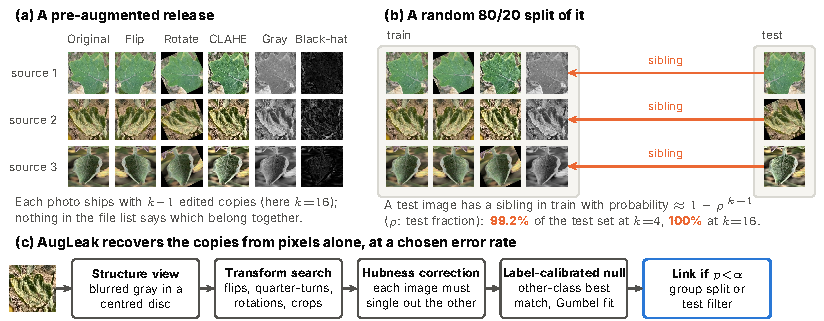
\includegraphics[width=\linewidth]{figs/fig1_concept.pdf}
  \caption{\textbf{The problem and our audit.} (a) Many public image datasets ship each photograph with $k-1$ edited copies and do not record which files belong together. (b) A random split then places a copy of almost every test image in the training set (Proposition~\ref{prop:exposure}). (c) AugLeak recovers copy relationships from pixels alone, at a user-chosen false-link rate.}
  \label{fig:concept}
\end{figure}



\section{Introduction}
\label{sec:intro}

Much applied computer-vision work starts from a public dataset that someone has already augmented: to reach a target size, every photograph ships with rotated, flipped, recoloured and filtered copies, and nothing records which copies belong together (Figure~\ref{fig:concept}a). The user then draws a random 80/20 split, trains, and reports test accuracy.

This paper shows that the number obtained this way measures very little, and that it can be wrong in either direction. The first error is leakage. With $k$ copies per photograph and test fraction $\rho$, a test image has a sibling in the training set with probability $\approx1-\rho^{k-1}$ (Proposition~\ref{prop:exposure}). At $k=4$ that is $99.2\%$ of the test set; at $k=16$ it is all of it, and the test score becomes, up to a weight of $3\times10^{-11}$, an accuracy on images the model has already seen in another guise (Proposition~\ref{prop:decomp}). The second error is that the test images are themselves edited copies, so even a leak-free split scores the model on filtered images that no deployment will see. On a controlled release built from CIFAR-10, a frozen-feature 1-NN classifier reports \numWeakKnnRep{} accuracy where the same model reaches \numWeakKnnFresh{} on fresh photographs; with stronger edits, the reported number falls \emph{below} the true one (Figure~\ref{fig:inflation}).

The obvious repair, recovering the groups with a near-duplicate detector, is harder than it looks. Released copies are deliberately dissimilar: an edge map of a leaf is closer, in an ImageNet embedding, to the edge maps of \emph{other} leaves than to its own original. And removing leakage needs complete groups: a group cut into two fragments still leaks with probability $1-\rho$ (Proposition~\ref{prop:frag}). On two real releases with known groups, splitting by the groups found by any detector we tried, including ours, leaves more than $90\%$ of test images with a sibling in training.

Yet the damage is not where nominal exposure suggests. Inflation is concentrated on test images whose closest training sibling is close in the model's own representation; siblings that are hard to match are also hard to exploit (Figure~\ref{fig:exploit}). A detector therefore does not need complete groups to be useful: splitting by the groups it finds removes most of the inflation when its similarity views match the release's edits (Section~\ref{sec:protocol}).

\paragraph{Contributions.}
\begin{itemize}[leftmargin=1.2em,itemsep=1pt,topsep=2pt]
\item \textbf{Theory of pre-augmented splits.} Exact exposure probabilities, the decomposition of reported accuracy into seen and unseen parts, and a fragmentation result showing why pairwise de-duplication does not remove leakage (Section~\ref{sec:theory}).
\item \textbf{Measurement.} On a controlled release with fresh ground-truth test images and on two real releases, we measure inflation across augmentation strength, copies per image, data size, classifier and backbone, and show the error can have either sign (Section~\ref{sec:inflation}).
\item \textbf{AugLeak}, a metadata-free sibling detector with an approximately calibrated error rate: a structure view robust to photometric filters, transform search, hubness correction and an extreme-value null derived from class labels (Section~\ref{sec:method}). On both real releases with ground-truth groups it has the highest average precision of all methods we tested (Section~\ref{sec:detect}).
\item \textbf{An evaluation of metadata-free protocols} showing when detected-group splits recover the oracle accuracy and why test filtering does not, and an \textbf{audit} of six public collections that finds repeat shots filed as independent photographs, test images duplicated in training (some under another label; half of one MRI test set) and radiographs filed under two patient identifiers (Sections~\ref{sec:protocol}--\ref{sec:audit}). Code and an auditing tool are released.
\end{itemize}

\section{Related work}
\label{sec:related}

\paragraph{Leakage.}
Leakage has been formalised for data mining~\citep{kaufman2012leakage} and catalogued as a cause of irreproducible results across applied fields~\citep{kapoor2023leakage,lones2024pitfalls}. Image-level instead of subject-level splits inflate accuracy for brain MRI~\citep{yagis2021mri} and retinal OCT~\citep{tampu2022oct}, and COVID-19 radiograph models suffered from many such pitfalls~\citep{roberts2021pitfalls}. \citet{gerz2025augmentation} show with two detection case studies that augmenting before splitting inflates mAP, and \citet{babu2024automotive} detect leakage between consecutive frames of driving video. These works measure leakage when the grouping is known. We study the case where it is not: we quantify why random splits of pre-augmented releases are nearly uninformative and can err in either direction, show that pair-level de-duplication does not remove the leak, and give a calibrated, metadata-free audit.

\paragraph{Duplicates in benchmarks and corpora.}
\citet{barz2020cifair} found near-duplicates of test images in the CIFAR training sets; \citet{recht2019imagenet} showed accuracy drops on freshly collected test sets; \citet{ramos2025leakage} measure exact and near-identical overlap within and across vision datasets; \citet{northcutt2021pervasive} audit test-set label errors. Web-scale de-duplication uses embeddings~\citep{abbas2023semdedup,webster2023laion,oquab2024dinov2} or hashing~\citep{lee2022dedup}, and copy detection learns edit-robust descriptors~\citep{pizzi2022sscd}. These target near-identical pairs at a fixed threshold. Pre-augmented releases differ in two ways that matter: copies are deliberately dissimilar, and removing leakage needs groups, not pairs. Our null turns the threshold into an error rate, using perceptual hashing~\citep{zauner2010phash}, ratio-test and local-scaling ideas~\citep{lowe2004sift,conneau2018csls} against hubs~\citep{radovanovic2010hubs}, and extreme-value theory~\citep{coles2001evt}.

\section{Why a random split of a pre-augmented release measures almost nothing}
\label{sec:theory}

\paragraph{Setting.}
A \emph{pre-augmented release} contains $N$ images formed from $G$ source photographs, each released with $k-1$ transformed copies, so $N=Gk$. Copies of one source are \emph{siblings} and share its label; the release does not record sibling identity. A user draws a uniformly random split with $n$ training images and test fraction $\rho=1-n/N$, trains a model $f$, and reports its test accuracy. The quantity of interest is the accuracy $a_U$ on images whose source was never seen, which is what a deployment on new photographs experiences.

\begin{proposition}[Exposure]\label{prop:exposure}
For a test image $x$ of a size-$k$ group, the probability that at least one sibling of $x$ is in the training set is
\begin{equation}
q(N,n,k) \;=\; 1-\binom{N-k}{n}\Big/\binom{N-1}{n} \;=\; 1-\prod_{j=1}^{k-1}\frac{N-n-j}{N-j}\;\approx\; 1-\rho^{\,k-1}.
\label{eq:exposure}
\end{equation}
\end{proposition}
\emph{Proof.} Conditioned on $x$ being in the test set, the training set is a uniformly random $n$-subset of the other $N-1$ images; $x$ is unexposed iff all $n$ are drawn from the $N-k$ non-siblings. The product form follows by expanding the binomials, and each factor tends to $\rho$ as $N\to\infty$. \hfill$\square$

With $\rho=0.2$, a release with $k=4$ exposes $99.2\%$ of its test set, and one with $k=16$ all but a fraction $\rho^{15}\approx3\times10^{-11}$. Exposure does not shrink as the dataset grows.

\begin{proposition}[What the reported number weighs]\label{prop:decomp}
Let $a_L$ and $a_U$ be the accuracies of $f$ on exposed and unexposed test images. The random-split accuracy is
\begin{equation}
\mathrm{acc}_{\text{random}} \;=\; q\,a_L + (1-q)\,a_U,
\qquad
\frac{\partial\,\mathrm{acc}_{\text{random}}}{\partial a_U}=1-q\approx\rho^{\,k-1}.
\label{eq:decomp}
\end{equation}
\end{proposition}
The identity is exact on any realised split (total probability over the exposure indicator). For $k\geq4$ the reported accuracy is, to within a percent, an estimate of $a_L$, the accuracy on images the model has seen in another guise; more test data does not help, because the unexposed part of the test set is empty in expectation.

\paragraph{De-duplicating is not the same as de-leaking.}
A natural fix is to recover the sibling groups with a near-duplicate detector and split by detected group. The next result shows why this is harder than near-duplicate detection is usually evaluated to be.

\begin{proposition}[Fragmentation]\label{prop:frag}
Suppose a detector partitions a true sibling group into $m$ fragments, and a group-aware split assigns each detected component to the test set independently with probability $\rho$. Then every member of that group that lands in the test set is exposed with probability $1-\rho^{\,m-1}$.
\end{proposition}
\emph{Proof.} The member's own fragment is in test; it is unexposed iff each of the other $m-1$ fragments is also in test. \hfill$\square$

Exposure after a detected-group split depends only on how many pieces each group is cut into, not on how many sibling pairs were found: a detector that finds every pair except those of one hard copy per group ($87.5\%$ of pairs at $k=16$) leaves that copy as a singleton ($m=2$), still exposed with probability $0.8$. Pairwise precision and recall, the standard near-duplicate metrics, are the wrong objective for removing leakage; group completeness is the right one, and it is far harder (Section~\ref{sec:detect}).

\paragraph{Exposure is not the same as exploitation.}
\Eqref{eq:decomp} also shows what matters: the inflation is $q\,(a_L-a_U)$, so an exposed sibling only inflates the score if the model can use it. A heavily filtered copy (an edge map, a black-hat transform) may be as foreign to the model as an unseen photograph. Section~\ref{sec:inflation} finds that inflation is indeed concentrated on close siblings, so a detector should be judged by the inflation it leaves, not by nominal exposure (Section~\ref{sec:protocol}).

\section{How wrong is the reported number?}
\label{sec:inflation}

\paragraph{Data.}
\emph{CIFAR-Aug} is a controlled pre-augmented release: $2{,}000$ CIFAR-10 training photographs~\citep{krizhevsky2009cifar}, each with $15$ edited copies at three strengths (weak: colour and flips; medium: plus rotations and crops; strong: plus one or two filters; Appendix~\ref{app:data}). Because the sources are known, we can also score every model on $3{,}000$ \emph{fresh} CIFAR-10 test photographs: the accuracy a deployment would see. \emph{Leaf-A} ($600$ sources $\times$ $15$ variants) and \emph{Leaf-B} ($850\times16$) are real public releases of field-crop leaf photographs, three classes each, whose file names encode the source; their variants include geometric edits and heavy filters (Figure~\ref{fig:concept}a). In \emph{COVID-CXR}~\citep{cohen2020covid} groups are patients; we use $699$ frontal radiographs of $424$ patients (COVID-19 vs.\ other findings).

\paragraph{Models.}
We use frozen ImageNet backbones (MobileNetV3-Large~\citep{howard2019mobilenetv3} in the main text, EfficientNet-B0~\citep{tan2019efficientnet} in Appendix~\ref{app:backbones}) with two heads that bracket how strongly a model can exploit a sibling: a 1-nearest-neighbour classifier (pure memory) and an $\ell_2$-regularised linear probe. Appendix~\ref{app:finetune} adds full fine-tuning. Every number is a mean over at least three seeds; the seed controls the split.

\begin{figure}[t]
  \centering
  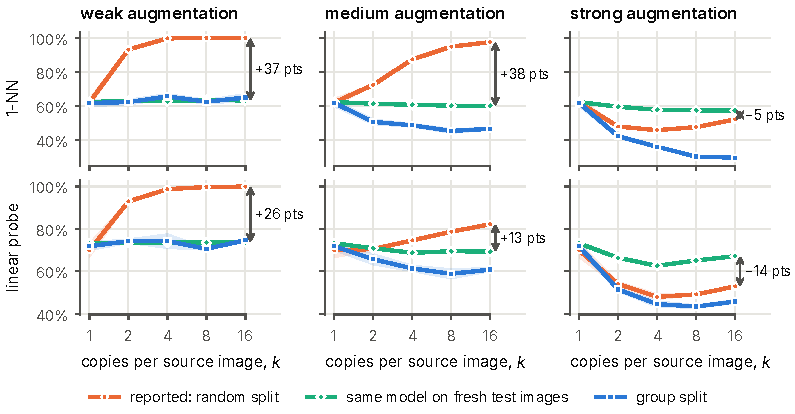
\includegraphics[width=\linewidth]{figs/fig_inflation.pdf}
  \caption{\textbf{Reported accuracy can be far above or below the truth.} CIFAR-Aug, $2{,}000$ sources, frozen MobileNetV3. Orange: the number a paper would report (random split). Green: the same model scored on fresh CIFAR-10 test photographs. Blue: a group split, which removes the leak but still tests on edited copies. Bands: 95\% intervals over seeds (often thinner than the line).}
  \label{fig:inflation}
\end{figure}

\paragraph{The error has two sources and either sign.}
Measured exposure matches \Eqref{eq:exposure} (Appendix Table~\ref{tab:exposure}): $100\%$ on both leaf releases and on CIFAR-Aug for $k\ge8$, \numCovidQ{} on COVID-CXR. Figure~\ref{fig:inflation} separates the two errors. With weak edits the reported 1-NN accuracy reaches \numWeakKnnRep{} while the same model scores \numWeakKnnFresh{} on fresh photographs; the linear probe is inflated from \numWeakLpFresh{} to \numWeakLpRep{}. Exposure saturates by $k=4$ (Proposition~\ref{prop:exposure}), yet the reported accuracy keeps rising with $k$ as more copies of each test image enter training, and the gap is larger for smaller releases: with medium edits the linear-probe gap is \numSizeGapSmall{} points for $500$ sources and \numSizeGapLarge{} for $2{,}000$ (Appendix Table~\ref{tab:datasize}). With strong edits the sign flips: the test set is now dominated by filtered images that are harder than real photographs, and the reported linear-probe accuracy (\numStrongLpRep{}) is \emph{below} the fresh accuracy (\numStrongLpFresh{}). A group split (blue) removes the leak but inherits this second bias; scoring the group split on the unedited member of each test group recovers the fresh accuracy (Appendix~\ref{app:orig}). The reported number is therefore not even a bound: it is a mixture of an optimistic and a pessimistic error whose balance depends on how the release was made.

\paragraph{Real releases.}
On the real data (Appendix Table~\ref{tab:real}), random splits overstate group-split accuracy by \numLeafALpGap{} (Leaf-A) and \numLeafBLpGap{} (Leaf-B) points for the linear probe and by up to \numLeafBKnnGap{} points for 1-NN; patient leakage in COVID-CXR adds \numCovidLpGap{} points. End-to-end fine-tuning, which can memorise individual images~\citep{zhang2017rethinking,feldman2020memorization}, does not remove them (Appendix~\ref{app:finetune}): on CIFAR-Aug (medium, $k=8$) a fine-tuned MobileNetV3 reports \numFtCMedRandom{} under a random split but reaches \numFtCMedRandomFresh{} on fresh photographs (EfficientNet-B0: \numFtCMedEffRandom{} vs.\ \numFtCMedEffRandomFresh{}; 3 seeds), and on Leaf-B the random split reports \numFtLeafBRandom{} where the group split gives \numFtLeafBGroup{}, understating the error rate about \numFtLeafBErrRatio{}-fold.


\paragraph{Which siblings are exploited?}
Figure~\ref{fig:exploit} bins test images of a random split by the cosine similarity, in the model's own embedding, between each image and its closest training sibling. When that sibling is dissimilar, accuracy is close to, or on the leaf releases even below, the group-split accuracy: these are mostly heavily filtered copies, not helped by their siblings. As the sibling gets closer, accuracy climbs steeply towards $100\%$. A detector therefore need not find every sibling, only the ones the model can use.

\begin{figure}[t]
  \centering
  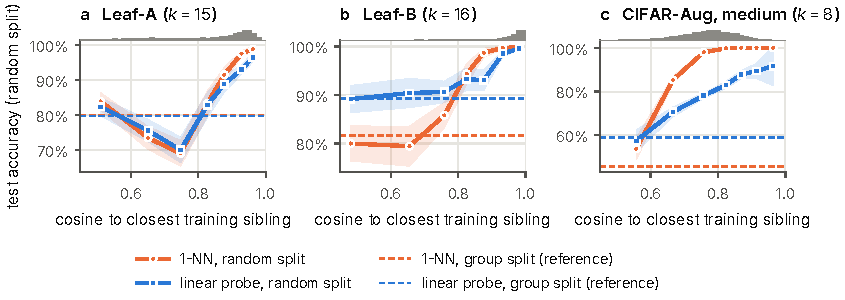
\includegraphics[width=\linewidth]{figs/fig_exploit.pdf}
  \caption{\textbf{Inflation comes from close siblings.} Accuracy of test images in a random split, binned by the cosine between each image and its closest training sibling in the probe's embedding (bins with $\ge30$ images; bands are 95\% binomial intervals; grey bars show how test images are distributed over the bins). Dashed lines: accuracy under a group split.}
  \label{fig:exploit}
\end{figure}

\section{AugLeak: recovering hidden siblings from pixels alone}
\label{sec:method}

AugLeak links two images when the evidence that they are copies of one photograph is strong enough at a user-chosen error rate $\alpha$. It needs only the images and their class labels. It is built from four parts (Figure~\ref{fig:concept}c), each answering a failure we observed in standard near-duplicate signals. The parts are generic: any similarity can be plugged in as a \emph{view}. By default AugLeak uses two pixel views, the structure view below and a 64-bit DCT perceptual hash~\citep{zauner2010phash} searched over the dihedral group, and combines them by the Bonferroni-adjusted minimum $p$-value; an optional third, semantic view is described in Section~\ref{sec:detect}.

\paragraph{1. A structure view that survives photometric edits.}
Released copies are often made by filters that rewrite intensities (CLAHE, thresholding, top-hat, grayscale, gamma) but leave the \emph{geometry} in place, and ImageNet embeddings group such copies by filter rather than by photograph (Section~\ref{sec:detect}). We therefore represent each image by a blurred grayscale thumbnail ($64\times64$, Gaussian $\sigma=1$, resampled to $32\times32$), restricted to a centred disc so that rotations do not move content in or out, mean-centred and $\ell_2$-normalised. The pair score is the correlation of the two vectors.

\paragraph{2. Transform search.}
Geometric copies are matched by maximising the correlation over a set $\mathcal{T}$ of query transforms: the eight elements of the dihedral group (quarter-turns and reflections) and rotations by $\pm15^\circ,\pm30^\circ,\pm45^\circ$ of the image and of its mirror, and a few crops:
$s_{ij}=\max_{t\in\mathcal{T}}\langle\phi(t(x_i)),\phi(x_j)\rangle$.

\paragraph{3. Hubness correction.}
In high dimension some images are close to everything~\citep{radovanovic2010hubs}; low-texture or dark copies are such hubs and generate many spurious matches. Following the local scaling idea of CSLS~\citep{conneau2018csls}, we standardise each score by the querying image's own score distribution, $z_{i\to j}=(s_{ij}-\mu_i)/\sigma_i$, where $\mu_i,\sigma_i$ are taken over images of \emph{other} classes, and keep the weaker direction, $z_{ij}=\min(z_{i\to j},z_{j\to i})$: a pair is only strong if each image singles out the other.

\paragraph{4. A label-calibrated null with extreme-value $p$-values.}
Label-preserving augmentation never moves a copy to another class, so the best match of image $i$ among other-class images, $m_i=\max_{j:\,y_j\neq y_i} z_{ij}$, is a draw from the distribution of the strongest \emph{unrelated} match. The $m_i$ are maxima, so we fit them with a Gumbel law~\citep{coles2001evt} and convert any pair score into an upper-tail $p$-value, $p_{ij}=1-\exp\!\big(-e^{-(z_{ij}-\hat\mu)/\hat\beta}\big)$. Two same-class images are linked when $p_{ij}<\alpha$. The fit extrapolates beyond the largest observed null score, so $\alpha$ can be set below $1/N$. Calibration rests on one assumption: that unrelated same-class pairs are not systematically more similar in the structure view than unrelated cross-class pairs. We test it empirically with ground-truth groups (Section~\ref{sec:detect}) rather than assume it.

\paragraph{Exact copies.} Byte-identical same-class files are always linked, since hubness correction can bury verbatim copies in a class whose images all look alike (Section~\ref{sec:audit}). In our benchmarks this touches only $15$ Leaf-A pairs, so Sections~\ref{sec:detect}--\ref{sec:protocol} report the statistical links alone.

\paragraph{Use and cost.}
Connected components of the links are detected groups, which can drive a group-aware split (Section~\ref{sec:protocol}). For $N$ images the structure view computes $|\mathcal{T}|\,N^2$ inner products of dimension $732$ (we use $|\mathcal{T}|=28$, adding centre and corner crops to the transforms above; Appendix~\ref{app:hyper}); for $N=13{,}600$ this takes a few minutes on two CPU cores and no GPU.

\section{Recovering siblings against known groups}
\label{sec:detect}

We evaluate on Leaf-A, Leaf-B and a CIFAR-Aug subset of $500$ sources, $50$ from each of the ten classes ($8{,}000$ images per strength), whose groups are known. Every method is turned into links the same way (hubness correction, label-calibrated null, $p<\alpha$), so the comparison isolates the similarity. Baselines are byte hashes, the perceptual hash~\citep{zauner2010phash} with and without dihedral search, and the frozen ImageNet embedding (with its dihedral orbit average). We also test a self-supervised \emph{invariant embedding}: a linear projection of the frozen embedding fitted on the release itself, which keeps directions that separate photographs and discards directions that a fixed, generic family of edits moves (a Fisher criterion with synthetic copies as classes; Appendix~\ref{app:invariant}). It uses no labels or groups, and the edit family is the same for every dataset.

\begin{table}[t]
\centering\small
\setlength{\tabcolsep}{4pt}
\caption{\textbf{Recovering siblings against known groups.} AP: average precision over all image pairs. Hit: share of images linked to at least one true sibling at $\alpha=10^{-3}$. Best per column in bold. File-name groups in Leaf-A/B miss repeat shots of the same leaf (Section~\ref{sec:audit}), so precision there is a lower bound.}
\label{tab:detect}
\begin{tabular}{@{}lcccccccccc@{}}
\toprule
 & \multicolumn{2}{c}{Leaf-A} & \multicolumn{2}{c}{Leaf-B} & \multicolumn{2}{c}{C-Aug weak} & \multicolumn{2}{c}{C-Aug medium} & \multicolumn{2}{c}{C-Aug strong} \\
\cmidrule(lr){2-3}\cmidrule(lr){4-5}\cmidrule(lr){6-7}\cmidrule(lr){8-9}\cmidrule(lr){10-11}
method & AP & hit & AP & hit & AP & hit & AP & hit & AP & hit \\
\midrule
pHash & 0.38 & 56 & 0.55 & 74 & 0.50 & \textbf{100} & 0.03 & 3 & 0.01 & 1 \\
pHash, dihedral search & 0.44 & 63 & 0.64 & 79 & \textbf{1.00} & \textbf{100} & 0.04 & 6 & 0.01 & 1 \\
ImageNet embedding & 0.03 & 8 & 0.20 & 11 & \textbf{1.00} & \textbf{100} & 0.62 & 43 & 0.07 & 5 \\
invariant embedding & 0.10 & 28 & 0.49 & 74 & \textbf{1.00} & \textbf{100} & 0.66 & \textbf{74} & 0.07 & \textbf{9} \\
structure view & 0.51 & 55 & 0.72 & 54 & \textbf{1.00} & 39 & 0.48 & 23 & \textbf{0.12} & 3 \\
AugLeak (structure + hash) & \textbf{0.57} & \textbf{81} & \textbf{0.76} & \textbf{83} & \textbf{1.00} & \textbf{100} & 0.42 & 26 & 0.09 & 4 \\
AugLeak (+ invariant) & 0.52 & 80 & -- & -- & \textbf{1.00} & \textbf{100} & \textbf{0.71} & 70 & 0.11 & \textbf{9} \\
\bottomrule
\end{tabular}
\end{table}


\paragraph{AugLeak is best on both real releases; ImageNet embeddings are worst.}
Table~\ref{tab:detect} and Figure~\ref{fig:detect} show that AugLeak's two pixel views together reach the highest average precision on Leaf-A (\numDetLeafApixAP{}) and Leaf-B (\numDetLeafBpixAP{}), ahead of either view alone and of perceptual hashing. The ImageNet embedding, a common tool for de-duplication, is the weakest method on both (AP \numDetLeafAsemAP{} and \numDetLeafBsemAP{}). Its failure is systematic, not noisy (Figure~\ref{fig:detect}e): filtered copies embed close to copies of \emph{other} photographs made with the same filter. The invariant projection repairs most of this from the release alone, but not for grayscale, rotation and morphological filters. Top-hat and black-hat copies defeat every method, and rotated copies are found less than half the time.

\paragraph{The right view depends on the edits.}
On CIFAR-Aug, where copies are random crops of $32\times32$ images, the pixel views are weak and the invariant view is strong. Adding it gives the best AP at medium strength (\numDetCmediumallAP{}). With weak edits every method that searches flips is near perfect. With strong edits (crops, rotations and filters at once, on tiny images) no method recovers most pairs.

\paragraph{Calibration.}
On CIFAR-Aug, AugLeak's pixel views are conservative (Figure~\ref{fig:detect}d): at every strength and $\alpha$, the share of images linked to a same-class non-sibling stays below $\alpha$. Adding the invariant view raises it to $5\times\alpha$ at $\alpha=10^{-4}$ (medium edits), because unrelated photographs of one class are close in an ImageNet embedding, which the label null does not see; we keep that view optional. The null also needs enough classes: on a three-class subset the pixel views' rate rose to $1.5$--$60\times\alpha$ (Appendix~\ref{app:hyper}). On the three-class leaf releases the rate is far higher, but most of these ``false'' links join different source photographs of the \emph{same physical leaf}, taken moments apart (Section~\ref{sec:audit}).

\paragraph{Pairs are not groups.}
As Proposition~\ref{prop:frag} predicts, splitting by detected components leaves most test images nominally exposed on every release, because groups fragment (Appendix Table~\ref{tab:resid}).

\begin{figure}[t]
  \centering
  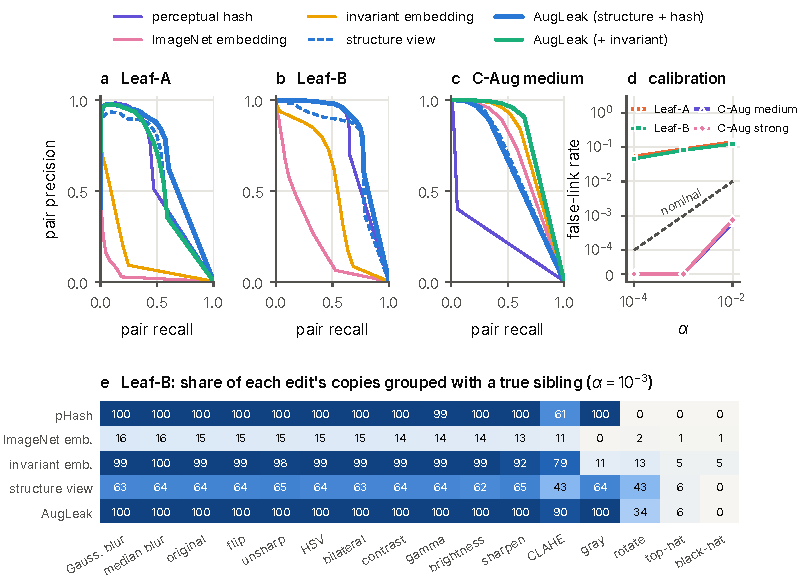
\includegraphics[width=\linewidth]{figs/fig_detect.pdf}
  \caption{\textbf{Sibling recovery with ground truth.} (a--c) Pairwise precision--recall over all image pairs (average precision in Table~\ref{tab:detect}). (d) Calibration of AugLeak: share of images linked to a same-class non-sibling, against the nominal $\alpha$; on the leaf releases most such links join repeat shots of the same leaf. (e) Leaf-B: share of each edit's copies that end up in a detected group with a true sibling, at $\alpha=10^{-3}$.}
  \label{fig:detect}
\end{figure}

\section{Evaluating a pre-augmented release without metadata}
\label{sec:protocol}

We now ask the practitioner's question: given only images and labels, how close to the oracle group-split accuracy can one get? We compare the naive random split with two protocols built on AugLeak links: a split by detected group (connected components), and \emph{test filtering}, which keeps the random split but scores only test images with no link to any training image. Table~\ref{tab:protocol} reports each protocol's error relative to the oracle.

\begin{table}[t]
\centering\small
\setlength{\tabcolsep}{4pt}
\caption{\textbf{Evaluating without metadata.} Error relative to the oracle group split, in accuracy points (mean of 3 seeds). Exposed: share of evaluated test images with a true sibling in training. Kept: share of the test set surviving filtering. AugLeak (structure + hash), or with the invariant view (+ inv.); $\alpha=10^{-2}$. CIFAR-Aug rows use the 500-source subset of Section~\ref{sec:detect}.}
\label{tab:protocol}
\begin{tabular}{@{}l rr rrr rrr@{}}
\toprule
 & \multicolumn{2}{c}{random split} & \multicolumn{3}{c}{detected-group split} & \multicolumn{3}{c}{random split + filter} \\
\cmidrule(lr){2-3}\cmidrule(lr){4-6}\cmidrule(l){7-9}
release & LP & 1-NN & LP & 1-NN & exposed & LP & 1-NN & kept \\
\midrule
Leaf-A & $+5.9$ & $+7.4$ & $-1.8$ & $-3.2$ & 93\% & $-11.9$ & $-15.9$ & 13\% \\
Leaf-A (+ inv.) & $+5.9$ & $+7.4$ & $-6.8$ & $-13.0$ & 93\% & $-14.2$ & $-17.0$ & 13\% \\
Leaf-B & $+7.7$ & $+14.6$ & $+1.1$ & $+3.1$ & 96\% & $-1.3$ & $+3.8$ & 13\% \\
CIFAR-Aug medium & $+36.3$ & $+56.4$ & $+31.4$ & $+52.5$ & 98\% & $+35.0$ & $+56.3$ & 57\% \\
CIFAR-Aug medium (+ inv.) & $+36.3$ & $+56.4$ & $+9.1$ & $+23.3$ & 60\% & $+25.4$ & $+51.0$ & 15\% \\
CIFAR-Aug strong & $+16.3$ & $+29.0$ & $+15.5$ & $+27.8$ & 100\% & $+15.3$ & $+27.5$ & 90\% \\
CIFAR-Aug strong (+ inv.) & $+16.3$ & $+29.0$ & $+14.9$ & $+26.0$ & 100\% & $+12.8$ & $+22.8$ & 82\% \\
\bottomrule
\end{tabular}
\end{table}


\paragraph{Detected-group splits remove most of the inflation, when the views match the edits.}
On Leaf-A the detected-group split moves the linear-probe error from \numProtLeafAnaiveErr{} to \numProtLeafAdgroupErr{} points, even though \numProtLeafAdgroupExp{} of its test images remain nominally exposed. The siblings it fails to separate are the dissimilar ones, which Figure~\ref{fig:exploit} shows the model cannot use. On CIFAR-Aug with medium edits the pixel views miss the cropped copies and the split barely helps (\numProtCmediumdgroupErr{}); adding the invariant view, which does match crops, brings the error from \numProtCmediumnaiveErr{} to \numProtCmediumInvdgroupErr{}. The cost of a view that does not match the release is over-linking: on Leaf-A the invariant view merges unrelated groups and the error overshoots to \numProtLeafAInvdgroupErr{}. With strong edits on tiny images, no configuration recovers enough siblings to matter.

\paragraph{Filtering is not a fix.}
Filtering removes the exposed test images that are easiest to match, and those are also the easiest to classify; what survives is a small and unrepresentative remainder (\numProtLeafAfilterKept{} of the Leaf-A test set), and its error relative to the oracle is \numProtLeafAfilterErr{} points. A test set that shrinks this much is a diagnostic: the release cannot support a random-split estimate.

\paragraph{Recommendation.}
Split by detected groups, choose views by inspecting the release (pixel views for filters and flips, the invariant view for crops), and report the detector's operating point. None of this replaces metadata: the only reliable protocol is a split by the groups the dataset creator knew, scored on the unedited member of each test group (Appendix Table~\ref{tab:orig}).

\section{Auditing public releases}
\label{sec:audit}

We ran AugLeak on the official or customary splits of six public image collections and inspected the highest-ranked candidate pairs by eye. In Fruits-360, $8\%$ of test images are nearby frames of a training image's capture sequence (Appendix~\ref{app:fruits}). Figure~\ref{fig:audit} shows examples and Appendix Table~\ref{tab:audit} summarises the counts. All inspected pairs and our judgements are released.

\begin{figure}[t]
  \centering
  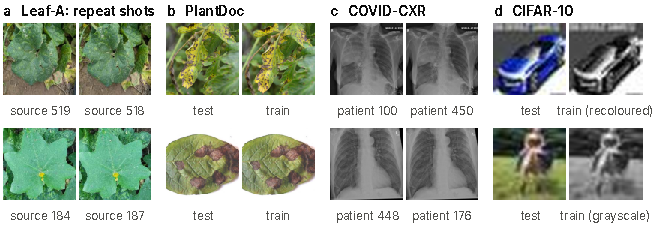
\includegraphics[width=\linewidth]{figs/fig_audit.pdf}
  \caption{\textbf{Examples from the audit}, all confirmed by inspection. (a) Two ``independent'' source photographs that show the same leaf. (b) PlantDoc test images also in training (lower pair: late blight in test, early blight in training). (c) One radiograph filed under two patient identifiers. (d) CIFAR-10 test images whose recoloured or grayscale copy is in the training set.}
  \label{fig:audit}
\end{figure}

\paragraph{Repeat shots defeat file-name groups.}
In both leaf releases, distinct source photographs are often the same physical leaf photographed again moments later. Among the $60$ highest-ranked cross-source pairs of canonical copies, we judged \numRepAyes{} (Leaf-A) and \numRepByes{} (Leaf-B) to show the same leaf; AugLeak links \numRepAlinked{} of Leaf-A's $600$ and \numRepBlinked{} of Leaf-B's $850$ sources to another source at $\alpha=10^{-2}$. A split by file-name group is therefore itself leaky. In each release one source photograph also appears under two classes (Table~\ref{tab:audit}).

\paragraph{PlantDoc.}
Eight of the $236$ official test images~\citep{singh2020plantdoc} ($3.4\%$) are byte-identical to a training image \emph{with a different label} (e.g.\ ``corn gray leaf spot'' in training, ``corn leaf blight'' in test). Among the $40$ top-ranked same-class pairs, \numPDyes{} more test photographs ($5.5\%$) also appear in training, often re-cropped or re-watermarked: at least \numPDtotal{} of the test set is compromised. A linear probe scores \numPDaccDup{} on these and \numPDaccRest{} on the rest.

\paragraph{COVID-19 radiographs.}
In COVID-CXR~\citep{cohen2020covid}, $62.5\%$ of frontal radiographs share a patient with another image, and an image-level split overstates patient-level accuracy by \numCovidLpGap{} (linear probe) and \numCovidKnnGap{} points (1-NN). Patient identifiers are not complete groups either: the top-ranked cross-patient pairs include three radiographs filed under two patient identifiers.

\paragraph{Brain MRI.}
In the official split of a widely used brain-tumour MRI collection~\citep{bhuvaji2020brain}, \numBTexact{} of the \numBTntest{} test images (\numBTexactPct{}), all labelled ``no tumour'', are byte-identical to training images. Hubness correction buried three quarters of them, hence AugLeak's exact-copy rule (Section~\ref{sec:method}). In all it flags \numBTflag{} test images (\numBTflagPct{}) at $\alpha=10^{-2}$, against \numBTcross{} linked to another class, where no copy should exist; all \numBTyes{} top-ranked non-identical pairs we inspected show the same slice. A linear probe scores \numBTaccFlag{} on flagged images and \numBTaccClean{} on the rest: the official \numBTaccAll{} is largely a score on seen slices.

\paragraph{CIFAR-10.}
\numCifarText{}

\section{Discussion and limitations}
\label{sec:discussion}

Dataset creators should release originals, keep source identifiers in file names, check for repeat shots and publish a group-aware split; users should never split such a release at the image level. \emph{Limitations.} We did not test large models beyond a small fine-tuning study (Appendix~\ref{app:finetune}). AugLeak's calibration depends on its views and on the number of classes; it assumes label-preserving edits, never recovers complete groups and misses many combined edits on tiny images. Duplicates were judged by eye.


\subsection*{AI use statement}
Generative AI tools were used extensively in this work: to help design the experiments, to write and debug the analysis code, to draft and edit the text, and to produce the figures. They also helped search the related literature; every reference was then verified against its original source. All numbers in the paper are produced by the released code from the released data and were checked against the result files. The visual inspection of candidate duplicate pairs in Section~\ref{sec:audit} was performed with AI assistance; every inspected pair and judgement is released so that it can be checked. The authors reviewed all AI-assisted work and take full responsibility for the content, claims and artifacts of this paper.

\subsection*{Ethics statement}
The audit concerns public datasets. Finding duplicates or label conflicts in a release is not a judgement of its creators: pre-augmenting a dataset is common practice, and the problems we describe arise from how downstream users split it. We contacted no individuals and used no personal data beyond what the public releases contain. COVID-CXR is a public collection of radiographs from published case reports and websites; we report only aggregate statistics and file names that are already public.

\subsection*{Reproducibility statement}
All experiments run on two CPU cores without a GPU. The code builds every manifest from the public releases, regenerates CIFAR-Aug deterministically, extracts features with fixed public ImageNet weights, and recreates every table and figure; seeds are fixed and listed. Appendix~\ref{app:data} gives dataset sources and preprocessing, and Appendix~\ref{app:hyper} gives all hyperparameters.


\bibliography{refs}
\bibliographystyle{iclr2027_conference}

\appendix
\section{Data and preprocessing}
\label{app:data}

\paragraph{CIFAR-Aug.} From the CIFAR-10 training set we draw $200$ images per class with a fixed seed. Each source receives $16$ variants per strength; variant $0$ is the untouched image. \emph{Weak}: brightness, contrast and saturation each scaled by a factor in $[0.85,1.15]$, then a horizontal flip with probability $0.5$. \emph{Medium}: flip ($p=0.5$), rotation uniform in $[-20^\circ,20^\circ]$, a square crop covering $75$--$100\%$ of the side at a random position resized back to $32\times32$, then colour factors in $[0.7,1.3]$. \emph{Strong}: as medium with rotation up to $30^\circ$, crops down to $60\%$ and colour factors in $[0.6,1.4]$, followed by one or two filters drawn from grayscale, Gaussian blur, sharpen, equalise, solarise, posterise, edge enhancement, quarter-turn, vertical flip and a per-channel intensity shift. The \emph{fresh} pool holds $300$ images per class from the CIFAR-10 test set. Generation is deterministic (seeded per source and strength).

\paragraph{Leaf-A and Leaf-B.} Two public releases of field photographs of crop leaves. Leaf-A has $9{,}000$ images: $600$ source photographs in three classes, each released with $15$ variants named \texttt{v1}--\texttt{v15}; \texttt{v1} appears to be the unedited photograph and the others include colour and contrast changes, grayscale, thresholding, edge maps, rotation and flips. Leaf-B has $13{,}600$ images: $850$ source photographs in three classes, each with $16$ named variants (Original, Flip, Rotate, Brightness, Contrast, Gamma, HSV, CLAHE, Grayscale, Gaussian and median blur, bilateral filter, sharpen, unsharp mask, top-hat, black-hat). In both releases the source identifier is part of the file name, which is what gives us ground-truth groups. To preserve double-blind review we do not name the releases here; they will be cited in the final version.

\paragraph{PlantDoc.} The official train ($2{,}342$) and test ($236$) folders of the classification release~\citep{singh2020plantdoc}: $28$ classes, $27$ of which occur in the test folder.

\paragraph{COVID-CXR.} From the metadata of the public collection~\citep{cohen2020covid} we keep X-ray images in the \texttt{images} folder with a frontal view (PA, AP, AP supine, AP erect) and a non-empty finding: $699$ images of $424$ patients. The label is COVID-19 versus any other finding; the group is the patient identifier.

\paragraph{CIFAR-10.} The official $50{,}000$/$10{,}000$ split.

\paragraph{Brain MRI.} The official \texttt{Training} ($2{,}870$) and \texttt{Testing} ($394$) folders of the four-class collection of \citet{bhuvaji2020brain} (glioma, meningioma, pituitary tumour, no tumour). Probes use frozen MobileNetV3 features at $160$ pixels.

\paragraph{Fruits-360.} The official \texttt{Training} and \texttt{Test} folders~\citep{muresan2018fruits} for $15$ classes (apple Braeburn, avocado, banana, cherry, kiwi, lemon, mango, orange, peach, pear, pineapple, pomegranate, strawberry, tomato, walnut): $7{,}759$ training and $2{,}600$ test images. Probes use frozen MobileNetV3 features at $112$ pixels.

\section{Hyperparameters}
\label{app:hyper}

\paragraph{Features.} timm~\citep{wightman2019timm} MobileNetV3-Large (\texttt{mobilenetv3\_large\_100}) and EfficientNet-B0 with public ImageNet weights, classifier removed (global-pooled features). Inputs are resized (no crop) to $112$ (CIFAR), $128$ (leaf releases) or $160$ pixels (PlantDoc, COVID-CXR) and normalised with the model's statistics. The dihedral orbit average is the mean embedding over the eight dihedral transforms.

\paragraph{Probes.} Linear probe: multinomial logistic regression on standardised features, $\ell_2$ penalty $10^{-3}$ on the weights, full-batch L-BFGS (50 iterations, strong Wolfe line search). 1-NN and 5-NN use cosine similarity. Splits are 80/20; group splits assign whole groups at random to reach a 20\% share of groups.

\paragraph{AugLeak.} Grayscale thumbnails $64\times64$, Gaussian blur $\sigma=1$, resampled to $32\times32$, disc of radius $0.48$ of the side ($732$ pixels). Query transforms: $8$ dihedral elements; rotations by $\pm15^\circ,\pm30^\circ,\pm45^\circ$ of the image and its mirror; centre crops of $80\%$ and $65\%$ of the side of the image and its mirror; corner crops of $75\%$ ($28$ transforms). Hash view: the $64$-bit DCT perceptual hash of the $32\times32$ thumbnail, searched over the $8$ dihedral elements. Hubness statistics use all other-class images. The Gumbel null is fitted by maximum likelihood to the best other-class score of every image. Views are combined by the Bonferroni-adjusted minimum $p$-value. Byte-identical same-class files are linked regardless of score (MD5 of the file). The audits of Section~\ref{sec:audit} use the structure view alone with this rule; the released command-line tool also adds the hash view and so flags somewhat more (for the brain-MRI split, $250$ rather than $200$ test images at $\alpha=10^{-2}$).

\paragraph{Calibration and the number of classes.} An earlier version of our CIFAR-Aug benchmark drew its $500$ sources from three classes. There, the pixel views linked same-class non-siblings at $1.5$--$3.1\times\alpha$ for $\alpha=10^{-2}$ and $10$--$60\times\alpha$ for $\alpha=10^{-4}$, against less than $\alpha$ on the ten-class subset. With few classes, the other-class best matches that define the null come from too narrow a slice of the image distribution. On releases with few classes, such as the two three-class leaf releases, the nominal $\alpha$ should therefore be read as a lower bound on the false-link rate.

\section{Invariant embedding}
\label{app:invariant}

We draw $M=1{,}500$ images from the release, make two copies of each with a generic edit family (horizontal and vertical flips, quarter-turns, rotation up to $30^\circ$, crops of $55$--$100\%$, brightness/contrast/saturation factors in $[0.6,1.4]$, and up to two of grayscale, blur, sharpen, equalise, autocontrast, posterise, edge detection and inversion), and embed the originals and copies. With $E_0$ the original embeddings, $\Sigma_b$ is the covariance of $E_0$ and $\Sigma_w$ the covariance of the differences between copies of one image (both copies against the original and against each other, halved). We solve $\Sigma_b v=\lambda(\Sigma_w+\epsilon I)v$ with $\epsilon=10^{-3}\,\mathrm{tr}(\Sigma_w)/d$ and keep the top $128$ directions. The edit family is fixed before seeing any release and is the same for all datasets.

\section{Additional results}
\label{app:orig}
\label{app:backbones}

\begin{table}[t]
\centering\small
\caption{\textbf{Real releases.} Accuracy under a random split (what is usually reported) and under a split by true group (source photograph or patient), frozen MobileNetV3; mean $\pm$ s.d.\ over seeds. $q$: share of test images with a sibling in training under the random split.}
\label{tab:real}
\begin{tabular}{@{}lrrr cc cc@{}}
\toprule
& & & & \multicolumn{2}{c}{linear probe} & \multicolumn{2}{c}{1-NN} \\
\cmidrule(lr){5-6}\cmidrule(l){7-8}
release & images & groups & $q$ & random & group & random & group \\
\midrule
Leaf-A & 9,000 & 600 & 100\% & 85.5\,{\scriptsize$\pm$0.4} & 79.2\,{\scriptsize$\pm$2.2} & 87.4\,{\scriptsize$\pm$0.7} & 80.0\,{\scriptsize$\pm$0.1} \\
Leaf-B & 13,600 & 850 & 100\% & 96.8\,{\scriptsize$\pm$0.4} & 88.5\,{\scriptsize$\pm$1.1} & 96.1\,{\scriptsize$\pm$0.3} & 80.6\,{\scriptsize$\pm$2.3} \\
COVID-CXR & 699 & 424 & 57\% & 76.6\,{\scriptsize$\pm$2.8} & 70.9\,{\scriptsize$\pm$4.2} & 77.0\,{\scriptsize$\pm$2.8} & 68.2\,{\scriptsize$\pm$3.7} \\
\bottomrule
\end{tabular}
\end{table}

\begin{table}[h]
\centering\footnotesize
\setlength{\tabcolsep}{4pt}
\caption{Exposure under an 80/20 random split: \Eqref{eq:exposure} against the measured share of test images with a sibling in training (mean over seeds).}
\label{tab:exposure}
\begin{tabular}{@{}lrr@{}}
\toprule
release & predicted $q$ & measured $q$ \\
\midrule
CIFAR-Aug, $k=1$ & 0.00\% & 0.00\% \\
CIFAR-Aug, $k=2$ & 80.02\% & 80.58\% \\
CIFAR-Aug, $k=4$ & 99.20\% & 99.50\% \\
CIFAR-Aug, $k=8$ & 100.00\% & 100.00\% \\
CIFAR-Aug, $k=16$ & 100.00\% & 100.00\% \\
Leaf-A ($k=15$) & 100.00\% & 100.00\% \\
Leaf-B ($k=16$) & 100.00\% & 100.00\% \\
\bottomrule
\end{tabular}
\end{table}

\begin{table}[h]
\centering\footnotesize
\setlength{\tabcolsep}{4pt}
\caption{CIFAR-Aug ($k=16$, 2{,}000 sources): scoring the group split only on the unedited member of each test group recovers the accuracy on fresh photographs. Accuracy in \%, mean over 3 seeds.}
\label{tab:orig}
\begin{tabular}{@{}llrrrr@{}}
\toprule
edits & probe & random split & group split & group split, originals & fresh photographs \\
\midrule
weak & 1-NN & 100.0 & 64.9 & 64.6 & 62.3 \\
weak & linear & 100.0 & 74.6 & 74.7 & 73.3 \\
medium & 1-NN & 97.6 & 46.5 & 60.0 & 59.7 \\
medium & linear & 82.2 & 60.8 & 68.6 & 68.8 \\
strong & 1-NN & 52.0 & 29.5 & 56.9 & 57.1 \\
strong & linear & 52.9 & 45.8 & 69.1 & 66.8 \\
\bottomrule
\end{tabular}
\end{table}

\begin{table}[h]
\centering\footnotesize
\setlength{\tabcolsep}{4pt}
\caption{CIFAR-Aug with $k=16$: reported (random split) / true (fresh photographs) accuracy in \% as the number of source photographs grows; mean over 3 seeds. Smaller releases are inflated more.}
\label{tab:datasize}
\begin{tabular}{@{}llrrr@{}}
\toprule
edits & probe & 500 sources & 1,000 sources & 2,000 sources \\
\midrule
weak & linear & 100.0 / 69.6 & 100.0 / 71.9 & 100.0 / 73.7 \\
weak & 1-NN & 100.0 / 58.0 & 100.0 / 60.3 & 100.0 / 63.2 \\
medium & linear & 92.7 / 63.6 & 86.9 / 65.8 & 82.2 / 69.3 \\
medium & 1-NN & 98.4 / 54.8 & 98.0 / 57.7 & 97.6 / 60.0 \\
strong & linear & 54.2 / 55.2 & 52.0 / 60.4 & 52.9 / 67.2 \\
strong & 1-NN & 57.4 / 52.2 & 54.0 / 54.2 & 52.0 / 57.2 \\
\bottomrule
\end{tabular}
\end{table}

\begin{table}[h]
\centering\footnotesize
\setlength{\tabcolsep}{4pt}
\caption{Inflation on the real releases for two frozen backbones (accuracy in \%, mean over seeds).}
\label{tab:backbones}
\begin{tabular}{@{}lllrrr@{}}
\toprule
release & backbone & probe & random & group & gap \\
\midrule
Leaf-A & MobileNetV3-L & linear & 85.5 & 79.2 & $+6.3$ \\
Leaf-A & MobileNetV3-L & 1-NN & 87.4 & 80.0 & $+7.4$ \\
Leaf-A & EfficientNet-B0 & linear & 85.7 & 79.5 & $+6.2$ \\
Leaf-A & EfficientNet-B0 & 1-NN & 87.6 & 81.1 & $+6.5$ \\
Leaf-B & MobileNetV3-L & linear & 96.8 & 88.5 & $+8.4$ \\
Leaf-B & MobileNetV3-L & 1-NN & 96.1 & 80.6 & $+15.5$ \\
Leaf-B & EfficientNet-B0 & linear & 96.6 & 89.2 & $+7.3$ \\
Leaf-B & EfficientNet-B0 & 1-NN & 95.5 & 81.3 & $+14.2$ \\
\bottomrule
\end{tabular}
\end{table}

\begin{table}[h]
\centering\footnotesize
\setlength{\tabcolsep}{4pt}
\caption{Residual exposure after splitting by detected components (share of test images with a true sibling in training, mean over 5 splits) and image-level false-link rate, at three values of $\alpha$.}
\label{tab:resid}
\begin{tabular}{@{}llrrrrrr@{}}
\toprule
release & method & exp.\ $10^{-2}$ & $10^{-3}$ & $10^{-4}$ & false $10^{-2}$ & $10^{-3}$ & $10^{-4}$ \\
\midrule
Leaf-A & pHash & 100\% & 100\% & 100\% & 10.2\% & 5.0\% & 1.7\% \\
Leaf-A & pHash, dihedral search & 100\% & 100\% & 100\% & 8.3\% & 5.4\% & 1.8\% \\
Leaf-A & ImageNet embedding & 100\% & 100\% & 100\% & 17.6\% & 7.8\% & 3.1\% \\
Leaf-A & invariant embedding & 100\% & 100\% & 100\% & 36.7\% & 15.2\% & 4.1\% \\
Leaf-A & structure view & 96\% & 99\% & 99\% & 12.9\% & 7.2\% & 3.6\% \\
Leaf-A & AugLeak (structure + hash) & 91\% & 99\% & 100\% & 14.1\% & 8.8\% & 5.4\% \\
Leaf-A & AugLeak (+ invariant) & 95\% & 99\% & 100\% & 31.7\% & 14.2\% & 6.8\% \\
Leaf-B & pHash & 100\% & 100\% & 100\% & 9.5\% & 6.4\% & 1.4\% \\
Leaf-B & pHash, dihedral search & 99\% & 99\% & 100\% & 10.6\% & 4.1\% & 0.3\% \\
Leaf-B & ImageNet embedding & 100\% & 100\% & 100\% & 7.1\% & 3.0\% & 1.3\% \\
Leaf-B & invariant embedding & 96\% & 99\% & 100\% & 44.1\% & 24.7\% & 13.8\% \\
Leaf-B & structure view & 95\% & 97\% & 99\% & 11.0\% & 6.0\% & 2.3\% \\
Leaf-B & AugLeak (structure + hash) & 94\% & 98\% & 100\% & 12.4\% & 8.1\% & 4.6\% \\
C-Aug weak & pHash & 79\% & 79\% & 83\% & 0.0\% & 0.0\% & 0.0\% \\
C-Aug weak & pHash, dihedral search & 0\% & 0\% & 0\% & 0.0\% & 0.0\% & 0.0\% \\
C-Aug weak & ImageNet embedding & 0\% & 1\% & 13\% & 4.3\% & 0.6\% & 0.1\% \\
C-Aug weak & invariant embedding & 0\% & 0\% & 0\% & 6.9\% & 2.2\% & 0.4\% \\
C-Aug weak & structure view & 29\% & 61\% & 80\% & 0.0\% & 0.0\% & 0.0\% \\
C-Aug weak & AugLeak (structure + hash) & 0\% & 0\% & 0\% & 0.0\% & 0.0\% & 0.0\% \\
C-Aug weak & AugLeak (+ invariant) & 0\% & 0\% & 0\% & 3.8\% & 1.0\% & 0.2\% \\
C-Aug medium & pHash & 100\% & 100\% & 100\% & 0.1\% & 0.0\% & 0.0\% \\
C-Aug medium & pHash, dihedral search & 100\% & 100\% & 100\% & 0.1\% & 0.0\% & 0.0\% \\
C-Aug medium & ImageNet embedding & 82\% & 95\% & 98\% & 2.6\% & 0.5\% & 0.0\% \\
C-Aug medium & invariant embedding & 57\% & 82\% & 92\% & 2.5\% & 0.4\% & 0.1\% \\
C-Aug medium & structure view & 97\% & 100\% & 100\% & 0.3\% & 0.0\% & 0.0\% \\
C-Aug medium & AugLeak (structure + hash) & 98\% & 99\% & 100\% & 0.1\% & 0.0\% & 0.0\% \\
C-Aug medium & AugLeak (+ invariant) & 61\% & 85\% & 95\% & 0.9\% & 0.1\% & 0.1\% \\
C-Aug strong & pHash & 100\% & 100\% & 100\% & 0.2\% & 0.0\% & 0.0\% \\
C-Aug strong & pHash, dihedral search & 100\% & 100\% & 100\% & 0.2\% & 0.0\% & 0.0\% \\
C-Aug strong & ImageNet embedding & 100\% & 100\% & 100\% & 1.1\% & 0.1\% & 0.0\% \\
C-Aug strong & invariant embedding & 100\% & 100\% & 100\% & 1.5\% & 0.2\% & 0.1\% \\
C-Aug strong & structure view & 100\% & 100\% & 100\% & 0.0\% & 0.0\% & 0.0\% \\
C-Aug strong & AugLeak (structure + hash) & 100\% & 100\% & 100\% & 0.1\% & 0.0\% & 0.0\% \\
C-Aug strong & AugLeak (+ invariant) & 100\% & 100\% & 100\% & 0.6\% & 0.1\% & 0.0\% \\
\bottomrule
\end{tabular}
\end{table}

\begin{table}[h]
\centering\footnotesize
\setlength{\tabcolsep}{4pt}
\caption{Leaf-A: share of copies of each released variant that end up in a component with a true sibling ($\alpha=10^{-3}$). The release does not name its variants; v1 is the unedited photograph.}
\label{tab:variants}
\begin{tabular}{@{}lrrrr@{}}
\toprule
variant & pHash, dihedral search & ImageNet embedding & invariant embedding & structure view \\
\midrule
v1 & 100 & 24 & 86 & 56 \\
v2 & 100 & 0 & 2 & 56 \\
v3 & 42 & 0 & 1 & 33 \\
v4 & 42 & 0 & 1 & 78 \\
v5 & 100 & 15 & 47 & 55 \\
v6 & 100 & 14 & 38 & 56 \\
v7 & 100 & 11 & 25 & 55 \\
v8 & 32 & 0 & 0 & 97 \\
v9 & 32 & 0 & 0 & 97 \\
v10 & 1 & 0 & 0 & 16 \\
v11 & 1 & 0 & 0 & 16 \\
v12 & 100 & 20 & 69 & 55 \\
v13 & 100 & 18 & 62 & 54 \\
v14 & 0 & 7 & 7 & 54 \\
v15 & 100 & 24 & 85 & 55 \\
\bottomrule
\end{tabular}
\end{table}


\begin{table}[t]
\centering\small
\setlength{\tabcolsep}{4pt}
\caption{\textbf{Audit findings.} Counts of flagged items and how they were verified (byte identity, metadata, or our inspection of the top-ranked candidate pairs).}
\label{tab:audit}
\begin{tabular}{@{}llp{5.2cm}rl@{}}
\toprule
release & size & finding & count & verified \\
\midrule
Leaf-A & 600 sources & repeat shots of one leaf filed as different sources & 113 linked & 57/60 confirmed \\
Leaf-A &  & source photo filed under two classes & 1 & byte-identical \\
Leaf-B & 850 sources & repeat shots of one leaf filed as different sources & 117 linked & 52/60 confirmed \\
Leaf-B &  & source photo filed under two classes & 1 & byte-identical \\
PlantDoc & 236 test & test image in train with another label & 8 & byte-identical \\
PlantDoc &  & test photograph also in train (same label) & 13 & 13/40 top pairs \\
COVID-CXR & 699 images & images sharing a patient with another image & 437 & metadata \\
COVID-CXR &  & same radiograph under two patient ids & 3 pairs & 3/6 top pairs \\
CIFAR-10 & 10,000 test & test image near-duplicated in train & 118 flagged & 55/60 top pairs \\
Brain MRI & 394 test & test image byte-identical to a training image & 88 & byte-identical \\
Brain MRI &  & test slice near-duplicated in train & 112 flagged & 40/40 top pairs \\
Fruits-360 & 2,600 test & test frame of the same fruit, same capture sequence & 219 flagged & 40/40 sampled pairs \\
\bottomrule
\end{tabular}
\end{table}


\FloatBarrier
\section{Fruits-360}
\label{app:fruits}
In the official split of Fruits-360~\citep{muresan2018fruits} (15 classes), AugLeak flags \numFRflag{} of \numFRntest{} test images (\numFRflagPct{}) at $\alpha=10^{-3}$. Every flagged pair joins two frames with the same file-name prefix, that is, the same capture sequence of one rotating fruit, a median of six frames apart; all \numFRyes{} pairs we inspected show the same fruit in nearly the same pose. Here the leak does not change the score: a linear probe exceeds $99.9\%$ on flagged and unflagged images alike, because the task is saturated.


\FloatBarrier
\section{Fine-tuning}
\label{app:finetune}
\IfFileExists{tables/finetune.tex}{\begin{table}[h]
\centering\footnotesize
\setlength{\tabcolsep}{4pt}
\caption{End-to-end fine-tuning of ImageNet backbones (AdamW, one-cycle schedule, learning rate $10^{-3}$, batch 64, label smoothing 0.1, horizontal flips; CIFAR-Aug: $k=8$, $64$ px, 4 epochs; Leaf-B: $96$ px, 3 epochs). Accuracy in \%, mean $\pm$ s.d.\ over seeds. Fresh: the same model scored on fresh CIFAR-10 test photographs.}
\label{tab:finetune}
\begin{tabular}{@{}llrrrrr@{}}
\toprule
release & backbone & random & group & fresh (random-split) & fresh (group-split) & seeds \\
\midrule
CIFAR-Aug medium & MobileNetV3-L & 98.2\,{\scriptsize$\pm$0.4} & 69.7\,{\scriptsize$\pm$1.6} & 73.6\,{\scriptsize$\pm$0.3} & 72.3\,{\scriptsize$\pm$0.5} & 3 \\
CIFAR-Aug medium & EfficientNet-B0 & 98.8\,{\scriptsize$\pm$0.1} & 71.4\,{\scriptsize$\pm$2.8} & 75.0\,{\scriptsize$\pm$0.3} & 73.1\,{\scriptsize$\pm$0.1} & 3 \\
CIFAR-Aug weak & MobileNetV3-L & 100.0\,{\scriptsize$\pm$0.0} & 72.4\,{\scriptsize$\pm$1.1} & 73.0\,{\scriptsize$\pm$0.2} & 71.6\,{\scriptsize$\pm$1.0} & 3 \\
Leaf-B & MobileNetV3-L & 99.4\,{\scriptsize$\pm$0.1} & 92.8\,{\scriptsize$\pm$2.1} & -- & -- & 3 \\
\bottomrule
\end{tabular}
\end{table}
}{Fine-tuning results are pending.}


\end{document}
